% Options for packages loaded elsewhere
\PassOptionsToPackage{unicode}{hyperref}
\PassOptionsToPackage{hyphens}{url}
%
\documentclass[
  11pt,
]{article}
\title{Berkeley Unified Numident Mortality Database: Public
Administrative Records for Individual-Level Mortality
Research\footnote{The authors benefited from helpful discussions with
  Lynn Goodsell, Berkeley Human Mortality Database, Ugur Yildirim, Leora
  Lawton, and members of the CenSoc Workig Group. The original NARA
  Numident Records are available upon request.}}
\author{Joshua Goldstein\footnote{\href{mailto:josh.goldstein@berkeley.edu}{\nolinkurl{josh.goldstein@berkeley.edu}};
  Department of Demography, UC Berkeley}\\
Casey Breen\footnote{\href{mailto:caseybreen@berkeley.edu}{\nolinkurl{caseybreen@berkeley.edu}};
  Department of Demography, UC Berkeley}}
\date{15 December, 2021}

\usepackage{amsmath,amssymb}
\usepackage{lmodern}
\usepackage{setspace}
\usepackage{iftex}
\ifPDFTeX
  \usepackage[T1]{fontenc}
  \usepackage[utf8]{inputenc}
  \usepackage{textcomp} % provide euro and other symbols
\else % if luatex or xetex
  \usepackage{unicode-math}
  \defaultfontfeatures{Scale=MatchLowercase}
  \defaultfontfeatures[\rmfamily]{Ligatures=TeX,Scale=1}
\fi
% Use upquote if available, for straight quotes in verbatim environments
\IfFileExists{upquote.sty}{\usepackage{upquote}}{}
\IfFileExists{microtype.sty}{% use microtype if available
  \usepackage[]{microtype}
  \UseMicrotypeSet[protrusion]{basicmath} % disable protrusion for tt fonts
}{}
\makeatletter
\@ifundefined{KOMAClassName}{% if non-KOMA class
  \IfFileExists{parskip.sty}{%
    \usepackage{parskip}
  }{% else
    \setlength{\parindent}{0pt}
    \setlength{\parskip}{6pt plus 2pt minus 1pt}}
}{% if KOMA class
  \KOMAoptions{parskip=half}}
\makeatother
\usepackage{xcolor}
\IfFileExists{xurl.sty}{\usepackage{xurl}}{} % add URL line breaks if available
\IfFileExists{bookmark.sty}{\usepackage{bookmark}}{\usepackage{hyperref}}
\hypersetup{
  hidelinks,
  pdfcreator={LaTeX via pandoc}}
\urlstyle{same} % disable monospaced font for URLs
\usepackage[margin=1in]{geometry}
\usepackage{longtable,booktabs,array}
\usepackage{calc} % for calculating minipage widths
% Correct order of tables after \paragraph or \subparagraph
\usepackage{etoolbox}
\makeatletter
\patchcmd\longtable{\par}{\if@noskipsec\mbox{}\fi\par}{}{}
\makeatother
% Allow footnotes in longtable head/foot
\IfFileExists{footnotehyper.sty}{\usepackage{footnotehyper}}{\usepackage{footnote}}
\makesavenoteenv{longtable}
\usepackage{graphicx}
\makeatletter
\def\maxwidth{\ifdim\Gin@nat@width>\linewidth\linewidth\else\Gin@nat@width\fi}
\def\maxheight{\ifdim\Gin@nat@height>\textheight\textheight\else\Gin@nat@height\fi}
\makeatother
% Scale images if necessary, so that they will not overflow the page
% margins by default, and it is still possible to overwrite the defaults
% using explicit options in \includegraphics[width, height, ...]{}
\setkeys{Gin}{width=\maxwidth,height=\maxheight,keepaspectratio}
% Set default figure placement to htbp
\makeatletter
\def\fps@figure{htbp}
\makeatother
\setlength{\emergencystretch}{3em} % prevent overfull lines
\providecommand{\tightlist}{%
  \setlength{\itemsep}{0pt}\setlength{\parskip}{0pt}}
\setcounter{secnumdepth}{-\maxdimen} % remove section numbering
\newlength{\cslhangindent}
\setlength{\cslhangindent}{1.5em}
\newlength{\csllabelwidth}
\setlength{\csllabelwidth}{3em}
\newlength{\cslentryspacingunit} % times entry-spacing
\setlength{\cslentryspacingunit}{\parskip}
\newenvironment{CSLReferences}[2] % #1 hanging-ident, #2 entry spacing
 {% don't indent paragraphs
  \setlength{\parindent}{0pt}
  % turn on hanging indent if param 1 is 1
  \ifodd #1
  \let\oldpar\par
  \def\par{\hangindent=\cslhangindent\oldpar}
  \fi
  % set entry spacing
  \setlength{\parskip}{#2\cslentryspacingunit}
 }%
 {}
\usepackage{calc}
\newcommand{\CSLBlock}[1]{#1\hfill\break}
\newcommand{\CSLLeftMargin}[1]{\parbox[t]{\csllabelwidth}{#1}}
\newcommand{\CSLRightInline}[1]{\parbox[t]{\linewidth - \csllabelwidth}{#1}\break}
\newcommand{\CSLIndent}[1]{\hspace{\cslhangindent}#1}
\usepackage{subfig} \usepackage{adjustbox} \usepackage{pdflscape} \usepackage{float} \usepackage{booktabs} \newcommand{\blandscape}{\begin{landscape}} \newcommand{\elandscape}{\end{landscape}} \usepackage{rotating} \usepackage{pdfpages} \usepackage{caption}
\ifLuaTeX
  \usepackage{selnolig}  % disable illegal ligatures
\fi

\begin{document}
\maketitle
\begin{abstract}
With the release of Social Security application (SS-5), claim, and death
records, the National Archives and Records Administration (NARA) has
created a new administrative data resource for researchers studying
mortality. While much progress has been made in understanding the
demographic determinants of mortality in the United States using survey
data, the lack of population-level register data is a barrier to further
advances in mortality research. This publicly available dataset provides
researchers access to over 49 million individual-level mortality records
with demographic covariates and fine geographic detail, allowing for
high-resolution mortality research. In this paper, we document the
contents of this dataset, provide access to a cleaned and harmonized
version of the data, and discuss statistical methods for estimating
mortality differentials based on this deaths-only dataset. \newpage
\end{abstract}

{
\setcounter{tocdepth}{3}
\tableofcontents
}
\setstretch{1.5}
\newpage

\hypertarget{introduction}{%
\subsection{1. Introduction}\label{introduction}}

The Numerical Identification System (Numident) forms the backbone of the
U.S. Social Security Administration's recordkeeping system. For every
person with a Social Security number, the Numident tracks claims status,
date of birth (and, if applicable, death), as well as other background
information including birthplace, race, sex, and names of parents. In
2013, the Social Security Administration transferred a large portion of
their Numident records to the National Archives and Records
Administration (NARA). The public release of these records in 2019,
which we call ``NARA Numident,'' offers nearly complete coverage of
those who died from 1988 to 2005. In this paper, we describe the
contents of the publicly available records, introduce a cleaned and
harmonized version of the data, and show how the records can be used for
the study of mortality in the United States.

The NARA Numident is an individual-level dataset covering over 49
million people who have died. In addition to individual identifiers,
NARA Numident includes information on race, sex, birthplace, ZIP Code of
residence at the time of death, and administrative variables, such as a
person's age when they submitted their first Social Security application
and their total number of Social Security applications. There are no
direct measures of socioeconomic status in the NARA Numident. To
overcome this, the records can be linked using such individual
identifiers to obtain income and education covariates (Joshua R.
Goldstein et al. 2019). Identifiers include Social Security numbers as
well as names, birthplaces, and dates of birth. The death coverage is
nearly complete for deaths to persons age 65+ for the window of
1988-2005.

The public release of the NARA Numident makes it one of the first
administrative data sets on mortality that can be used by all
researchers. Previously, Social Security Numident records have been used
to study mortality by researchers employed by the Social Security
Administration (e.g., Waldron 2007) or collaborating with SSA
researchers (e.g., Mehta et al.~2016). Researchers using restricted
access IRS data have also carried out mortality research (Chetty et al.
2016). Our hope is that the public availability of this data will
encourage more mortality research using administrative records, enhance
the replicability and debate about results, and open up new avenues of
research.

Administrative data offers several advantages for the study of
mortality. The large sample sizes enable the comparison of ages, birth
cohorts, small subpopulations, and small geographic areas. The large
sample sizes also enable the study of mortality at the oldest ages, when
there are only a few survivors. An additional advantage is that the
public nature of the NARA Numident means that individual identifiers can
be used to link to other data with covariates of mortality. Since there
are no restrictions on the use of this public data, researchers can also
link records to their own restricted datasets.

The NARA Numident records pose a challenge for mortality estimation.
Because the dataset includes only those who have died, there is no
measure of survivorship. Traditional statistical methods relying on
exposure to risk are not appropriate. Instead, one needs to use methods
that rely on the distribution of deaths by age within cohorts. We
discuss these methods below and provide examples of their use.

The methods we provide here are also useful for researchers working with
the Social Security Death Master File (DMF), another publicly available
data resource for mortality research. The DMF was first made available
in 1988 and is extracted quarterly from the Numident (Hill and
Rosenwaike 2001). The file has been used by some researchers to study
mortality, particularly at older ages (Gavrilov and Gavrilova 2012).
While the DMF has high death coverage for the wider window of 1975 to
2005, it lacks most of the covariates available in the NARA Numident
records (Hill and Rosenwaike 2001).

We are also in the process of linking both the DMF and the NARA Numident
records to the complete count 1940 Census, to create a rich, publicly
linked administrative dataset for the study of mortality (Joshua R.
Goldstein et al. 2019).

\hypertarget{the-structure-and-content-of-the-nara-numident-records}{%
\subsection{2. The Structure and Content of the NARA Numident
Records}\label{the-structure-and-content-of-the-nara-numident-records}}

To illustrate the structure and content of the NARA Numident records, we
show the released records for the actress Lana Turner, who died in 1995,
and for Supreme Court Justice Thurgood Marshall, who died in 1993. For
Thurgood Marshall, we have one application and one death record. For
Lana Turner, we have one death record and four application records,
corresponding to name changes each time she got married.

\begin{landscape}
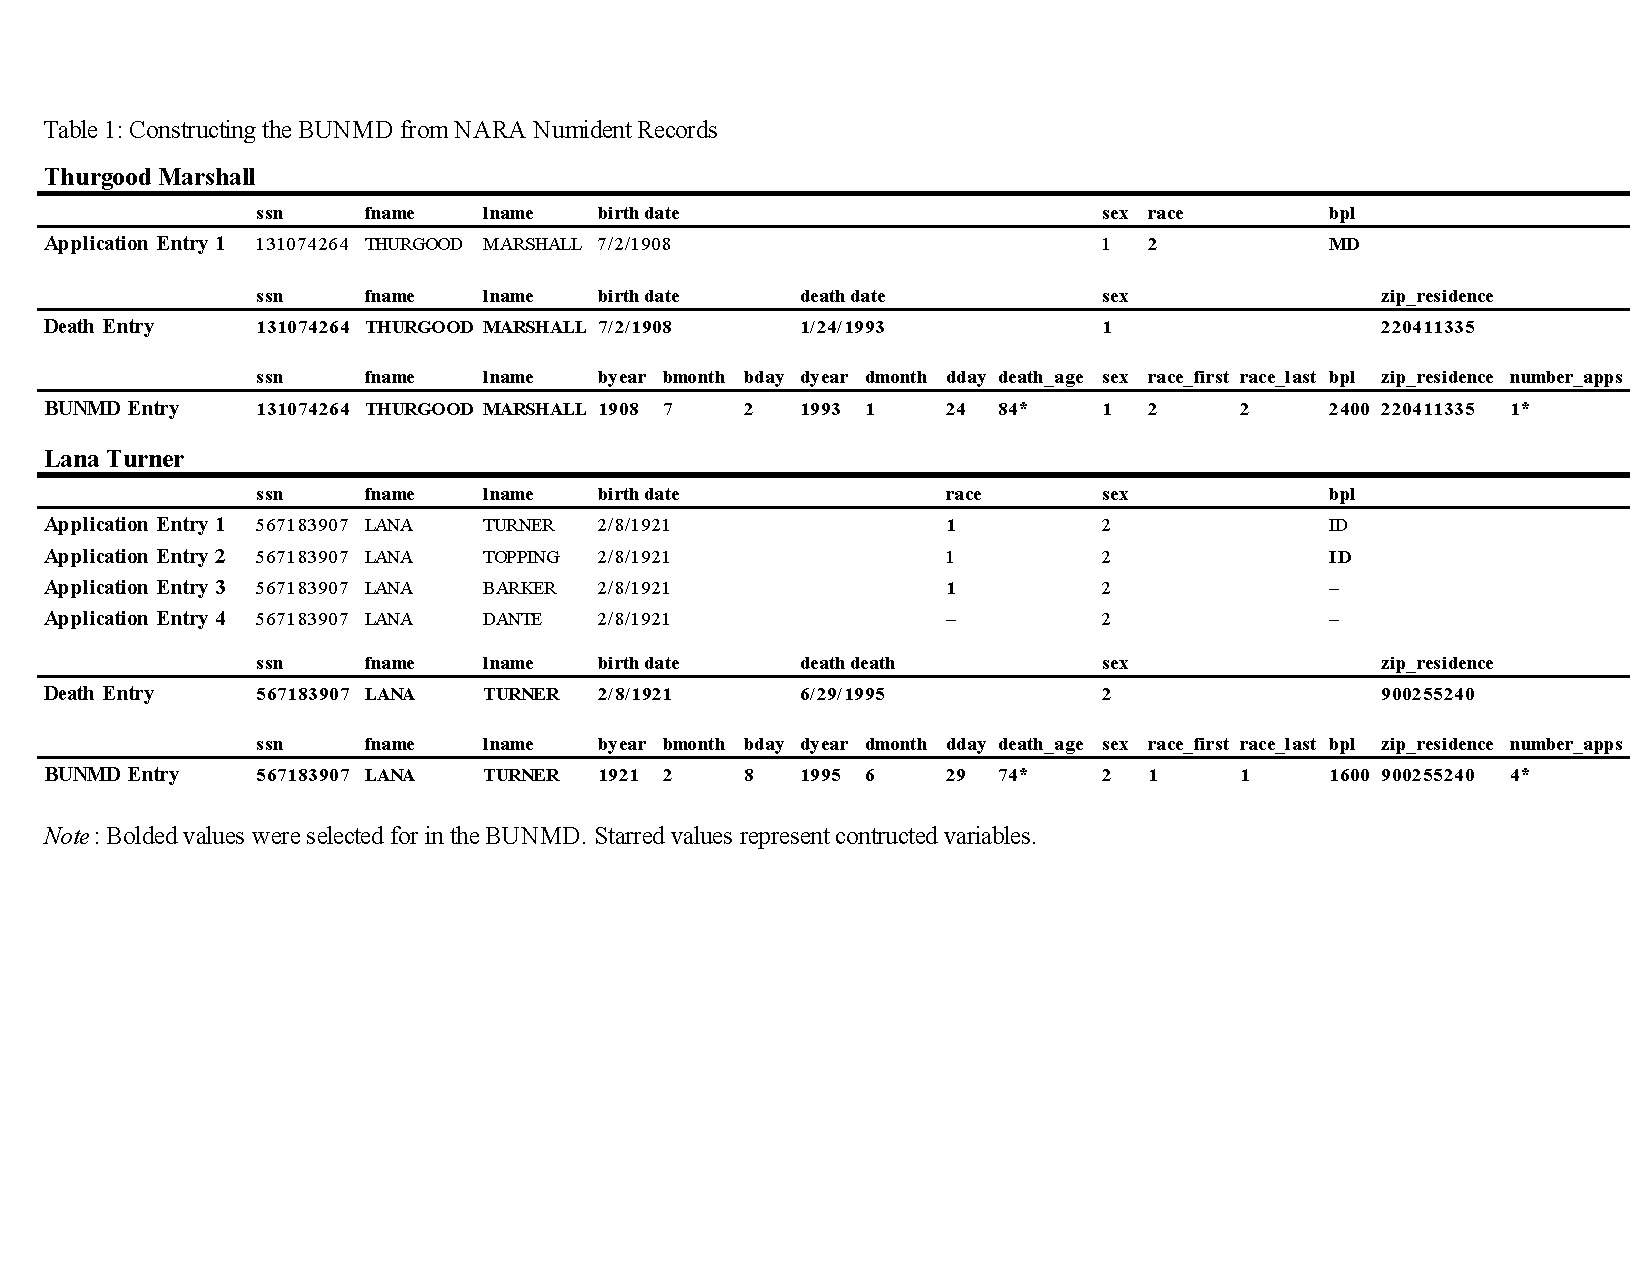
\includepdf[pages={-}, angle=90]{../illustrations/bunmd_chart.pdf}
\end{landscape}

The NARA Numident records contain three types of entries: application,
claim, and death. The application entries contained information
extracted from one of two forms, either the ``Application for a Social
Security Card'' or the ``Application for Social Security Account
Number.'' The application entries contain a person's full name, race,
sex, birthplace, date of birth, parents' full names, and other
administrative information. Individuals may submit additional
applications to replace a lost Social Security card, fix an error in a
previous entry, or make a name change. Claim entries contain a person's
full name, date of birth, sex, and whether the claim was a life claim or
a death claim. Some individuals may have multiple claim entries. The
Social Security Administration adds a new entry to the Numident when a
Social Security cardholder submits a new application or claim. New
entries never overlay old entries. Instead, a new entry is added to the
pre-existing Numident, ensuring that information is never overwritten.
Figure \ref{fig:number_entries} shows the distribution of application
and claim entries per person. In the NARA Numident records, 43.3\% of
persons have multiple application entries, 0.3\% of persons have
multiple claim entries, and 0\% have multiple death records.

\begin{figure}[H]
  \centering
  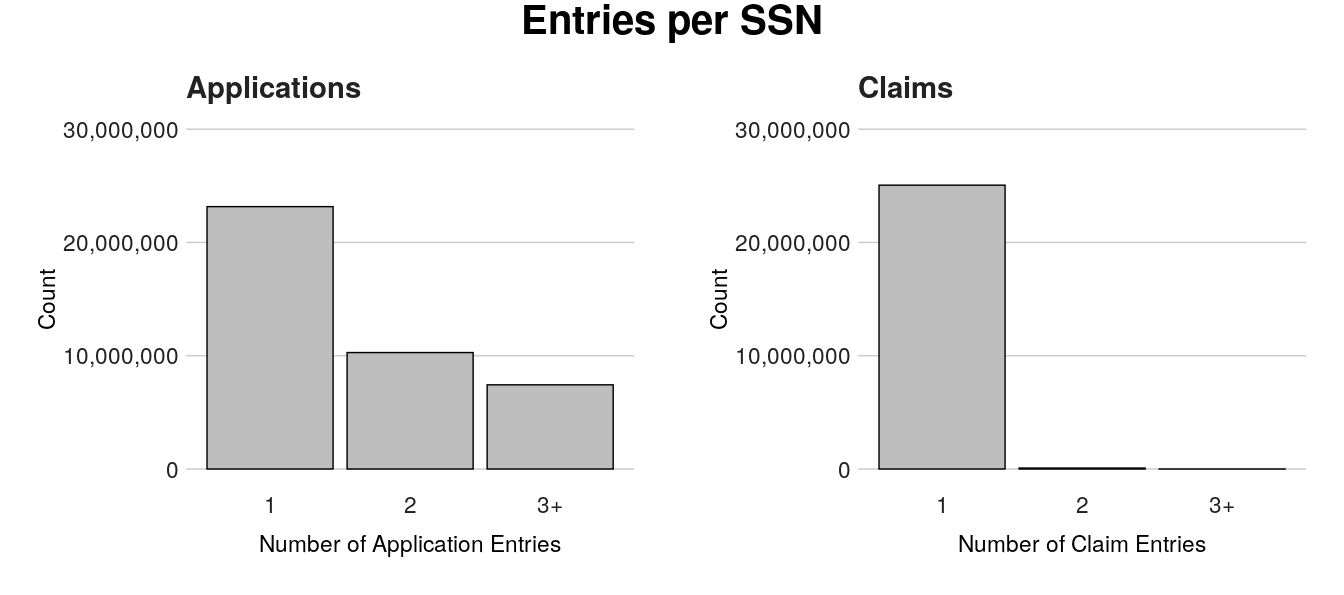
\includegraphics[width=7in]{../illustrations/entries_per_ssn.png}
  \caption{Number of entries per person for the Numident Application and Claim files.}
  \label{fig:number_entries}
\end{figure}

We introduce a cleaned and harmonized version of the NARA Numident
records: the Berkeley Unified Mortality Numident Database (BUNMD). This
file condenses the Numident death, application, and claim records into a
single file with one record per person. This file is available for
download at: \url{https://censoc-download.demog.berkeley.edu/}. The file
includes about 49 million records and 28 variables. It is 5.7GB in size.

The original NARA release contained 49,459,293 death record entries,
72,120,516 application entries for 40,870,455 unique persons, and
25,228,257 claim entries for 25,140,847 unique persons. To construct the
BUNMD, we first selected key variables from the death records. For each
record with a death entry, we added additional covariates from the
application and claim entries. For individuals with multiple application
or claim entries, we used a set of decision rules to reconcile
discrepant values across entries (see technical appendix for more
details). Finally, we constructed variables reporting (1) total number
of applications, (2) total number of claims, (3) age at first Social
Security application, and (4) state in which the Social Security number
was issued. Figure 2 shows the process for constructing the BUNMD. In
order to study name changes, race changes, and other features, the
original NARA Numident records are useful and are available upon
request.

\begin{figure}[H]
  \centering
  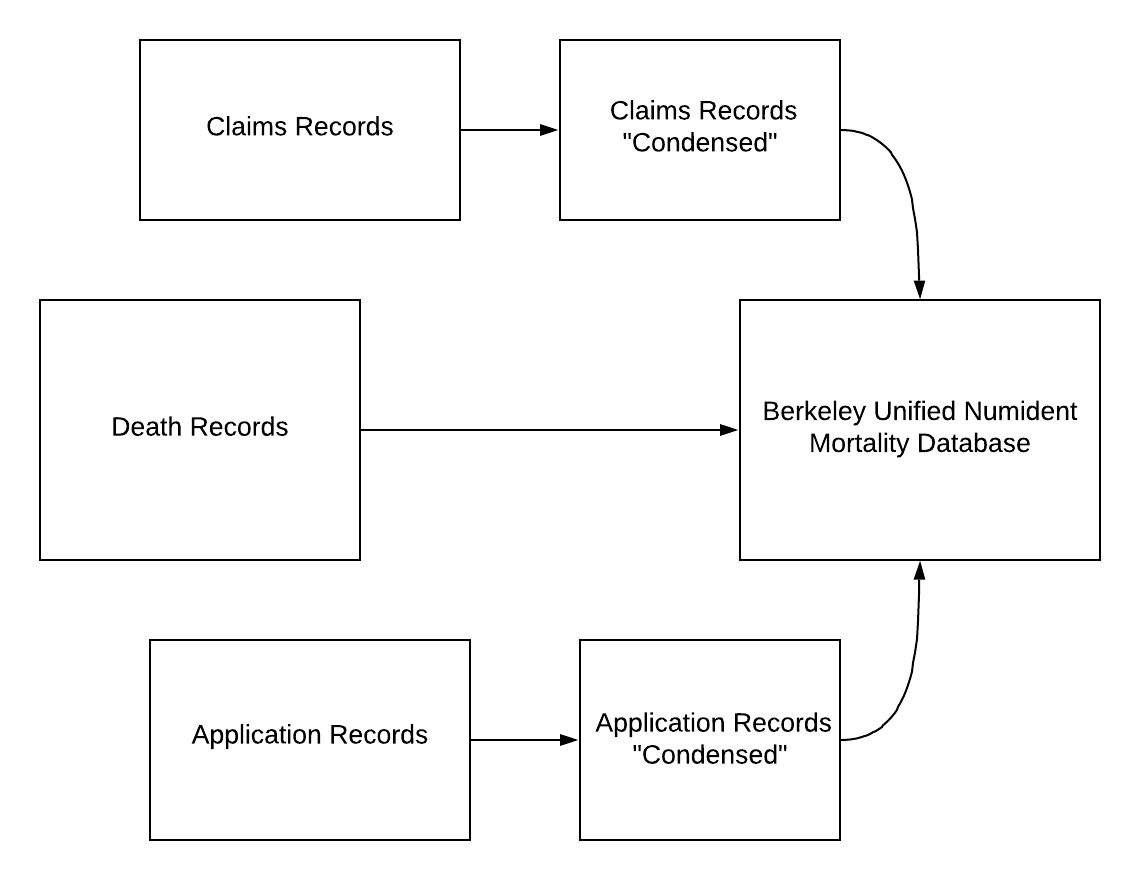
\includegraphics[width=5in]{../illustrations/numident_flowchart.png}
  \caption{Berkeley Unified Numident Mortality Database creation flowchart.}
  \label{fig:flowchart}
\end{figure}

\hypertarget{numident-coverage}{%
\subsubsection{2.1 Numident Coverage}\label{numident-coverage}}

The NARA Numident records are a subset of the complete Numident. One
challenge of working with the NARA Numident records is that the process
used by the Social Security Administration for selecting the records to
transfer to NARA for their public release is not well defined. The NARA
documentation states that the first transfer of records contained
``individuals with a verified death between 1936 and 2007 or who would
have been over 110 years old by December 31, 2007'' (Record Group 47
2019). However, there are many individuals who fit those criteria who
are not included in the dataset. Figure \ref{fig:bunmd_coverage}
compares the total number of deaths for persons age 65+ (when coverage
is highest) in the BUNMD to the Human Mortality Database (HMD). Death
Coverage is nearly complete between 1988 and 2005. Figure
\ref{fig:bunmd_lexis} shows the coverage visualized on an age-period
Lexis surface, an established demographic visualization technique
(Schöley and Willekens 2017). Each cell represents death coverage,
measured as the ratio of the total count of deaths in the BUNMD to the
total count of deaths in HMD for a given age and year.

We create two BUNMD samples with high death coverage. Sample 1 includes
deaths to persons age 65+, occurring between 1988 to 2005, from the
birth cohorts of 1900 to 1940. Sample 2 --- the ``complete case'' sample
--- is the subset of Sample 1 records with complete information on sex,
birthplace, and race. For each sample, we constructed inverse
probability weights to the Human Mortality Database on age at death,
year of birth, year of death, and sex.

\begin{figure}[H]
  \centering
  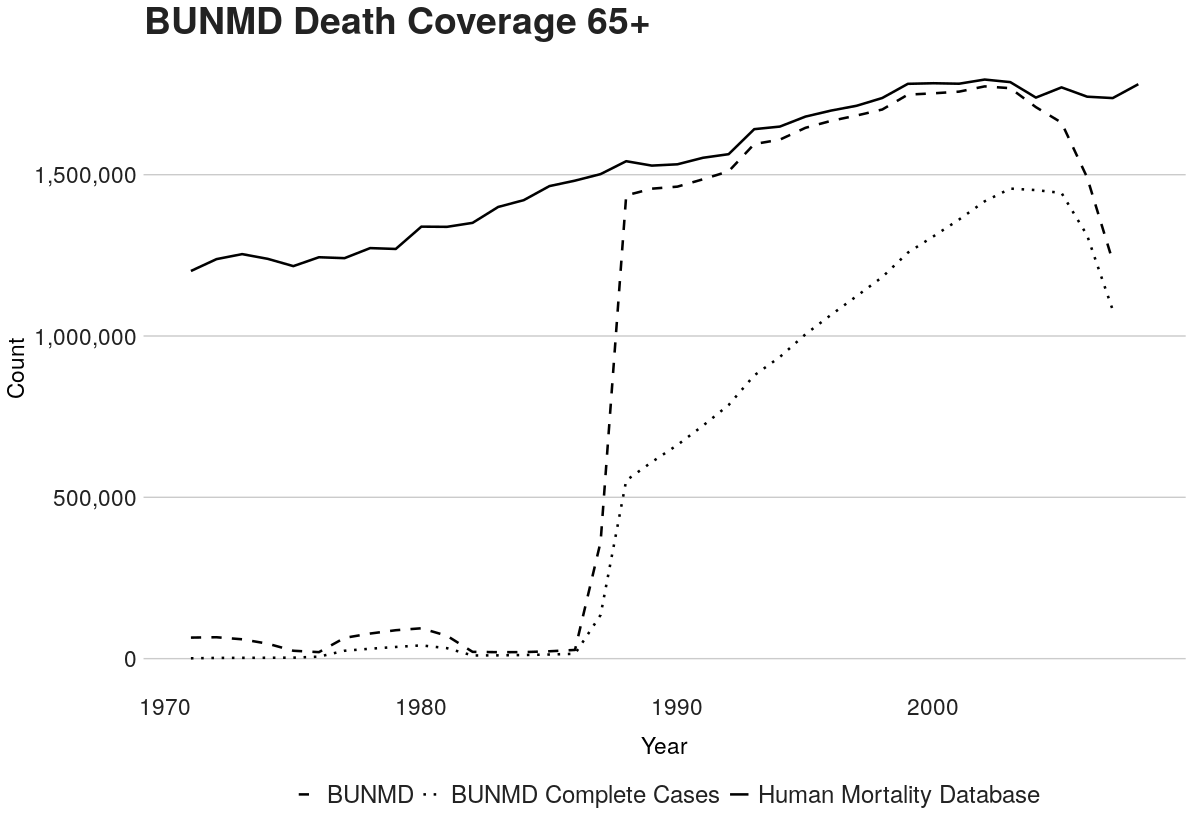
\includegraphics[width=6.5in]{../illustrations/bunmd_coverage.png}
  \caption{BUNMD Death Coverage for persons 65+. Coverage is most complete in the BUNMD for the window of 1988 to 2005.}
  \label{fig:bunmd_coverage}
\end{figure}

\begin{figure}[H]
  \centering
  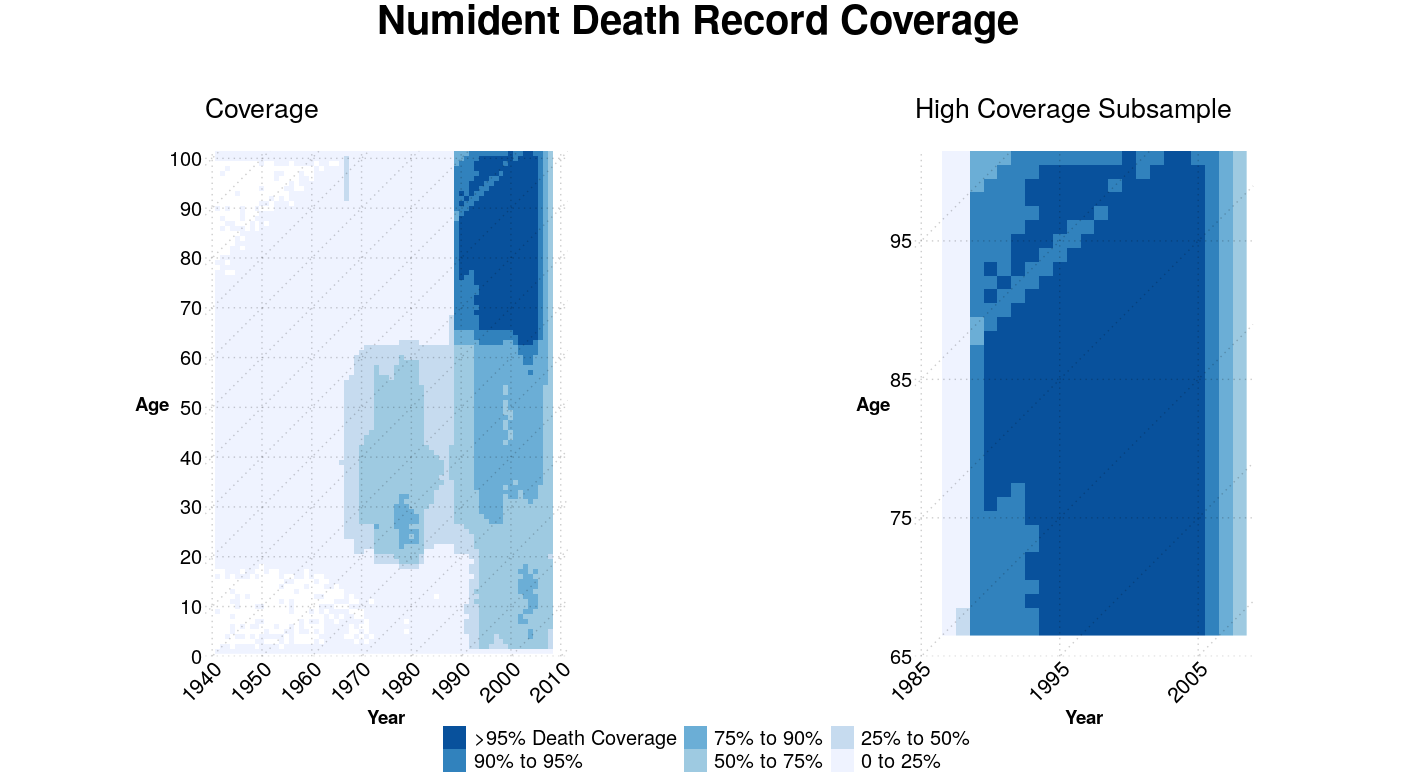
\includegraphics[width=7in]{../illustrations/lexis_combine_plot.png}
  \caption{Lexis diagrams of BUNMD death coverage. The left panel shows the BUNMD death coverage for 1940 to 2010. The right panel zooms in on age-period area where coverage is highest.}
  \label{fig:bunmd_lexis}
\end{figure}

\hypertarget{estimation-deaths-without-denominators}{%
\subsection{3. Estimation: Deaths without
Denominators}\label{estimation-deaths-without-denominators}}

The BUNMD file includes only individuals who have died. For extinct
cohorts (in which all members have died), it is possible to use
classical methods of ``extinct generations'' to calculate mortality
rates. These methods are appropriate for the cohorts born before 1900,
for which only a few survivors to age 105 will die after 2005. For later
cohorts, however, we have developed several different methods, which can
be chosen based on suitability for the research question of interest.

The first method is to fit parametric survival models (Gompertz and
Makeham), using maximum likelihood for doubly-truncated cohorts. The
second method is to use ordinary regression, inflating the observed
coefficients in order to account for truncation.

\hypertarget{method-1-parametric-survival-models-for-truncated-data}{%
\subsubsection{3.1 Method 1: Parametric Survival Models (for Truncated
Data)}\label{method-1-parametric-survival-models-for-truncated-data}}

Human mortality has a characteristic pattern in older ages. To a first
approximation --- first noticed by Benjamin Gompertz --- mortality
hazards rise exponentially with age.

\begin{equation}
h(x) = a \cdot e^{bx}
\end{equation}

The constant exponential rate of increase is most pronounced for the
ages of 70 to 90. At younger ages, between 40 and 70, mortality is often
somewhat higher than would be predicted by a Gompertz model. This was
first noted by Makeham, who suggested that adding a constant term would
be a better description of observed mortality:

\begin{equation}
h(x) = c + a \cdot e^{(bx)}
\end{equation}

Although there is still much debate, at older ages there may be a
leveling of mortality. Thus the logistic model has been introduced to
account for this leveling of mortality. For any parametric model, it is
possible to write down the likelihood given the deaths we observe. For
truncated cohorts, with known left truncation \(a\) and known right
truncation \(b\), we can define the conditional distribution to be

\begin{equation}
f_{trunc} = \frac{f_{\theta}(x)}{\int_a^b f_\theta (x)dx} = \frac{f_{\theta}(x)}{F_\theta (b) -F_\theta (a)  }
\end{equation}

with likelihood of

\begin{equation}
L(\theta | X) = \prod \frac{f_{\theta }(x_i) }{F_\theta (b) - F_{\theta} (a)}
\end{equation}

The estimates of the vector \(\theta\) of parameters can be obtained by
maximizing the likelihood, or, equivalently, the log-likelihood.

\hypertarget{method-2-ordinary-least-squares-regression}{%
\subsubsection{3.2 Method 2: Ordinary Least Squares
Regression}\label{method-2-ordinary-least-squares-regression}}

Regression on age at death is an easy and effective way to analyze the
Numident mortality data. Regression coefficients tell the effect of
covariates on the mean age at death. Because left and right truncation
ages vary by cohort, it is important to include fixed effect terms for
each year of birth. Models of the form:

\begin{equation}
  \text{Age\_at\_death = birth\_year\_dummy + covariates of interest}
\end{equation}

provide estimates of the effect of the covariates on the age of death in
the sample, controlling for birth cohort truncation effects.

Truncation, however, will tend to downwardly bias the estimated effects
of any covariates (Greene 2005). Truncation excludes the tails of the
distribution, thus reducing the average difference between groups; the
average differences between groups will be measured to be much smaller
if we exclude the tails of the distribution.

Simulation tells us that the magnitudes of the regression coefficients
need to be inflated by a factor of about 2 or 3 for many of the cohorts
that are covered by the Numident files. Figure
\ref{fig:regression_coeff} below gives the inflation factors for each
cohort, based on a simulation of a Gompertz distribution with M = 79.6
and b = 0.0826 (the values found by fitting to the untruncated cohort of
1910 using HMD data). The interpretation of these numbers is that a
regression coefficient of 0.5, as in the example comparing men and
women, found using the data from the cohort of 1910 (observed from 1988
to 2005) translates to an \(e65\) difference of 0.5 x 2.3 = 1.15 years.

\begin{figure}[H]
  \centering
  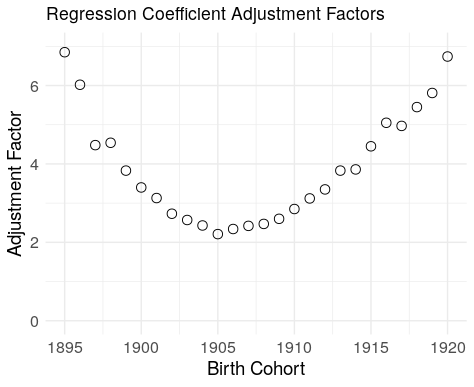
\includegraphics[width=6in]{../illustrations/regression_coefficient_adjustment.png}
  \caption{Regression coefficient adjustments for birth cohorts of 1895-1920 using baseline mortality schedule parameters $b = 1/10$ and $M = 84$}
  \label{fig:regression_coeff}
\end{figure}

Table 3 below shows the adjustment factors implied by different choices
of \(b\) and \(M\). The Human Mortality Database tells us that the birth
cohort of 1910 had a modal age of death of about 84 and a senescence
rate \(\beta\) of about 0.1. We recommend these as default choices. As
can be seen from the table, the adjustment factors are typically about
3, with much larger or smaller values found only in the extreme cases.
When the distribution of mortality is very compressed (high \(b\)) and
the modal age is young, the truncated tails are smaller and the
adjustment factor is closer to 2. When the distribution of mortality is
dispersed and the modal age is high, there is significant truncation,
and the adjustment factor can be 5 or even higher.

\begin{table}[H]
\begin{center}
\begin{tabular}{@{}lllllll@{}}
\toprule
    &                         &      &   &   $b$  &      &      \\
    &                         & 0.08 & 0.09 & 0.1 & 0.11 & 0.12 \\ \cmidrule(l){2-7} 
    & \multicolumn{1}{l|}{77} & 3.0    & 2.5  & 2.2 & 2.1  & 1.9  \\
    & \multicolumn{1}{l|}{78} & 3.2  & 2.7  & 2.4 & 2.2  & 2.0  \\
    & \multicolumn{1}{l|}{79} & 3.3  & 2.9  & 2.5 & 2.4  & 2.1  \\
    & \multicolumn{1}{l|}{80} & 3.5  & 3.0  & 2.8 & 2.4  & 2.2  \\
$M$ & \multicolumn{1}{l|}{81} & 3.9  & 3.2  & 2.8 & 2.5  & 2.4  \\
    & \multicolumn{1}{l|}{82} & 4.1  & 3.3  & 3.1 & 2.6  & 2.5  \\
    & \multicolumn{1}{l|}{83} & 4.3  & 3.7  & 3.2 & 2.9  & 2.6  \\
    & \multicolumn{1}{l|}{84} & 4.7  & 3.8  & 3.4 & 3.1  & 2.7  \\
    & \multicolumn{1}{l|}{85} & 4.9  & 3.8  & 3.6 & 3.2  & 2.9  \\
    & \multicolumn{1}{l|}{86} & 5.6  & 4.6  & 3.9 & 3.4  & 3.0    \\
    & \multicolumn{1}{l|}{87} & 6.1  & 5    & 4.2 & 3.7  & 3.3  \\
    &                         &      &      &     &      &      \\ \bottomrule
\end{tabular}
\end{center}
\caption*{Table 3: Regression coefficient adjustment factors for combined birth
cohorts 1895 to 1920, estimated by simulation for different
Gompertz parameter values $b$ and $M$.}
\end{table}

We recommend that users estimate the appropriate adjustment factor for
their analysis by specifying their choice of birth cohorts. The Gompertz
parameters can be left at their default values of \(\beta = 0.1\) and
\(M = 84\) unless there is a reason to override these values based on
external estimates.

Users can do their full statistical analysis, including hypothesis
testing and model selection, using regression on age at death with dummy
variables for year of birth. The adjustment factors can then be applied
when discussing the magnitude of results and comparing them to other
research findings. When greater precision is desired or comparisons
among cohorts are made, then more complex methods are needed.

We show regression results that report differences in mean age at death
observed in the truncated range of ages observable from 1988 through
2005. These differences will tend to be smaller the narrower the age
window considered.

For example, in the Figure \ref{fig:distribution_age_of_death} below, we
show two distributions of age at death in which population A has an life
expectancy at age 65 \((e65)\) of 18 years and population B has an
\(e65\) of 19 years.

\begin{figure}[H]
  \centering
  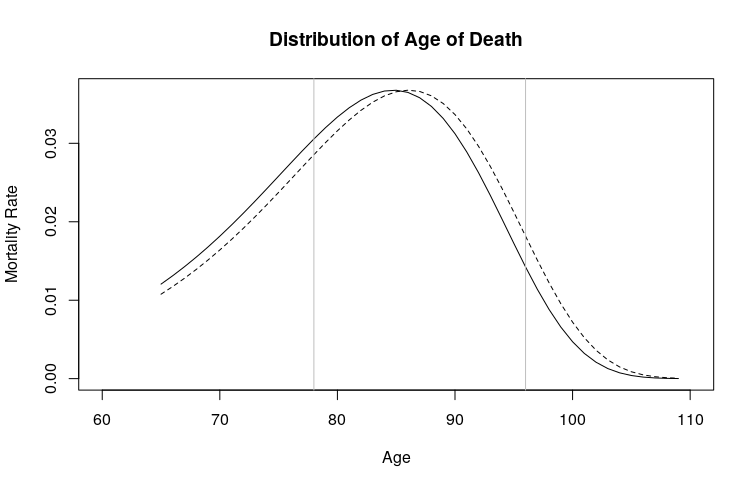
\includegraphics[width=6in]{../illustrations/distribution_age_of_death.png}
  \caption{Distributions of age of death for two populations. Gray lines represent hypothetical left and right truncation.}
  \label{fig:distribution_age_of_death}
\end{figure}

If we only observe deaths from ages 78 to 95, as we would for the cohort
of 1910, the difference in these truncated means will only be 0.358,
understating the \(e65\) difference by a factor of 2.79.

It is possible to estimate more sophisticated models that take into
account truncation and provide parametric and other model-based
estimates of the untruncated mortality distribution (Alexander 2018).
This is particularly useful for estimating changes in differences over
time, when the researcher does not want to confound time trends in the
effects of covariates with changing ages of truncation.

The regression approach has the advantage of being simpler, faster and
still easy to interpret. In order to translate regression results, we
recommend using a multiplicative adjustment factor, estimated using
simulation.

The simulation assumes two Gompertz mortality schedules with the same
senescence parameter \(b\) but differing modal ages of death \(M\), such
that their \(e65\) differs by one year. A function in the computer
language \({\tt R}\) , shown below, produces estimates of the adjustment
factor needed to translate differences in truncated means to differences
in \(e65\).

\begin{verbatim}
get.bunmd.adjust.factor(byear.vec,
                        b = 1/10, 
                        M = 84,
                        e65.diff = 1,
                        N = 1 * 10^6)
\end{verbatim}

The function allows the user to specify the set of birth cohorts,
e.g.~\texttt{byear.vec = 1895:1920}. It also allows the user to modify
the baseline mortality schedule parameters \(b\) and \(M\), as well as
the simulated difference in \(e65\). We find that the estimates are not
sensitive to the choice of difference in \(e65\), an encouraging result
that permits use of the same adjustment factor to a range of observed
differences in truncated means.

\hypertarget{case-studies}{%
\subsection{4. Case Studies}\label{case-studies}}

\hypertarget{the-old-age-mortality-of-the-foreign-born}{%
\subsubsection{4.1 The Old-Age Mortality of the
Foreign-Born}\label{the-old-age-mortality-of-the-foreign-born}}

The mortality of immigrants is often lower than natives, despite the
fact that many immigrants are often disadvantaged in terms of education
and income. The ``immigrant paradox'' has long been observed for Mexican
immigrants, one of the only immigrant groups of sufficient number to
produce accurate mortality measures from sample surveys. Recently, Mehta
et al. (2016) were able to use internal Social Security and Medicare
records, finding that a diverse set of immigrant groups had lower
mortality than natives.

Here, we first show how the BUNMD data can be used to confirm Mehta's
findings using publicly available data. We then take advantage of the
information on race to look at variation within Cuban immigrants. There
are many other topics that can be investigated relating to the mortality
of immigrants, including spatial patterns based on ZIP Code of residence
at the time of death and cultural variables that can be measured using
first and last names (Joshua R. Goldstein and Stecklov 2016).

In our analysis, we restrict ourselves to foreign-born individuals who
applied for Social Security cards before age 65 and before 1988. This
assures that the distribution of deaths we observe is not biased upwards
by immigrants arriving in the midst of our observation period. For the
study of race, we also restrict ourselves to individuals who recorded a
race before 1980, when the only options were ``White,'' ``Black,'' and
``Other.''

\hypertarget{country-of-birth-differences}{%
\subsubsection{4.2 Country-of-Birth
Differences}\label{country-of-birth-differences}}

To measure mortality differences by country of birth, we have chosen the
19 most common origins for immigrants in our sample who were born from
1910 to 1919. We fit a regression model separately for men and women,
with fixed effects for year of birth. This approach is aimed at reducing
compositional effects that stem from observing different ages of death
for each birth cohort.

Figure \ref{fig:immigrant_advantage} shows the difference in mean age of
death between natives and the foreign-born. Differences in mean ages in
the truncated sample understate differences in \(e65\). A good
approximation for translating the differences in the truncated sample
\(e65\) is to multiply the regression coefficients by about 4. We
discuss how such multiplicative factors can be estimated in the section
on Ordinary Least Squares Regression.

\begin{figure}[H]
  \centering
  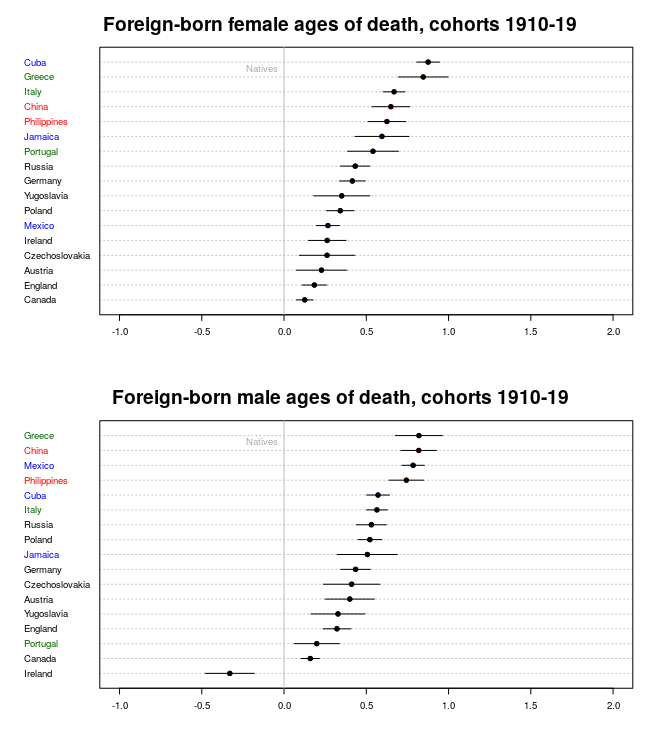
\includegraphics[width=6in]{../illustrations/immigrant_advantage_plot.png}
  \caption{Difference in mean age of death between natives and foreign-born.}
  \label{fig:immigrant_advantage}
\end{figure}

The large sample size gives us enough precision to see that there are
interesting patterns by individual country. Whereas Mehta reported
results for broader regions and found that immigrants from every region
had lower mortality than natives, the country-level estimates we report
here show that one group, Irish men, suffers a mortality disadvantage
relative to the native-born.

For both sexes, we see that the longest-lived groups come from a
remarkable variety of origins. A prominent explanation of immigrant
mortality advantage is selective migration: those who overcome obstacles
to migration are a select and quite healthy group. This theory has some
support from the pattern we see, with those born in countries that are
the farthest away, e.g., Greece, the Philippines, and China all being
among the longest lived, and those coming from relatively close, English
speaking countries (Canada, England, and Ireland) as having the smallest
longevity advantage. The Mexican case is interesting in that it is an
immediate geographic neighbor, but non-English speaking. Male migrants
from Mexico are among the longest lived, but female migrants from Mexico
do not appear to have a particularly large advantage over natives when
compared to other countries of origin.

There are many interesting avenues of research on the mortality
advantages of immigrants that could be explored with the Numident data.
Geographic variation, residence in higher and lower income areas,
residence in areas with other immigrants, differences by immigration
cohort (as proxied by age of first application for Social Security), and
racial and ethnic differences could all be pursued. In addition, first
and last names can also be analyzed for indications of ethnic diversity
within immigrant groups and for measures of acculturation (Joshua R.
Goldstein and Stecklov 2016).

\hypertarget{racial-differences-among-cuban-immigrants}{%
\subsubsection{4.3 Racial Differences Among Cuban
Immigrants}\label{racial-differences-among-cuban-immigrants}}

We saw above that Cuban immigrants are among the longest-living
subgroups in the United States. We can use the NARA Numident to further
explore whether immigrants from this racially diverse country differ in
their longevity in the United States, keeping in mind that racial
identity is self-identified on the Social Security SS-5 application. We
restrict ourselves to pre-1980 responses to the race question, when the
only options were White (N = 35,000), Black (N = 1,000), and Other (N =
800).

We report the results of a regression of age of death on race, sex, and
birth year in Table 3 below. We can see that Black Cuban immigrants died
earlier than White Cuban immigrants. The effect of -0.7 years in the
regression corresponds to an \(e65\) of about 3 years. There is not a
statistically significant difference between Cuban immigrants that
identified as Other and those who identified as White. The disadvantage
of Black Cuban immigrants is consistent with racial inequality in Cuba
and with the reception of Cubans in the United States (Newby and Dowling
2007).

This analysis could be extended by looking at the residential patterns
of Black and White Cuban immigrants in the United States. There are also
other immigrant origins, such as the Dominican Republic and Brazil that
are racially diverse. A deeper dive into the original SS-5 application
files may also reveal interesting patterns about who chooses a Hispanic
identity and when. For example, one could link the Numident records to
the 1940 Census, finding that those who change their identity from
Hispanic to White tend to have higher earnings and educational
attainment.

\begin{table}[] \centering 
  \caption{} 
  \label{} 
\begin{tabular}{@{\extracolsep{5pt}}lc} 
\\[-1.8ex]\hline 
\hline \\[-1.8ex] 
 & \multicolumn{1}{c}{\textit{Dependent variable:}} \\ 
\cline{2-2} 
\\[-1.8ex] & death\_age \\ 
\hline \\[-1.8ex] 
  Race: Black & $-$0.696$^{***}$ (0.159) \\ 
  Race: Other & 0.284 (0.159) \\ 
  Byear1895 & 7.354$^{**}$ (2.562) \\ 
  Byear1897 & 4.835 (3.574) \\ 
  Byear1898 & 8.932$^{***}$ (1.194) \\ 
  Byear1899 & 3.816 (2.027) \\ 
  Byear1900 & 6.660$^{***}$ (0.885) \\ 
  Byear1901 & 5.082$^{***}$ (1.010) \\ 
  Byear1902 & 4.273$^{***}$ (0.542) \\ 
  Byear1903 & 4.597$^{***}$ (0.394) \\ 
  Byear1904 & 4.661$^{***}$ (0.301) \\ 
  Byear1905 & 3.213$^{***}$ (0.253) \\ 
  Byear1906 & 2.522$^{***}$ (0.194) \\ 
  Byear1907 & 2.311$^{***}$ (0.174) \\ 
  Byear1908 & 1.352$^{***}$ (0.144) \\ 
  Byear1909 & 0.206 (0.122) \\ 
  Byear1911 & $-$0.425$^{***}$ (0.106) \\ 
  Byear1912 & $-$1.125$^{***}$ (0.112) \\ 
  Byear1913 & $-$1.873$^{***}$ (0.113) \\ 
  Byear1914 & $-$2.581$^{***}$ (0.118) \\ 
  Byear1915 & $-$3.444$^{***}$ (0.126) \\ 
  Byear1916 & $-$4.211$^{***}$ (0.129) \\ 
  Byear1917 & $-$5.105$^{***}$ (0.129) \\ 
  Byear1918 & $-$5.825$^{***}$ (0.127) \\ 
  Byear1919 & $-$6.728$^{***}$ (0.128) \\ 
  Byear1920 & $-$7.728$^{***}$ (0.128) \\ 
  Gender (Female) & 1.743$^{***}$ (0.049) \\ 
  Constant & 84.422$^{***}$ (0.082) \\ 
 \hline \\[-1.8ex] 
Observations & 39,852 \\ 
R$^{2}$ & 0.280 \\ 
Adjusted R$^{2}$ & 0.280 \\ 
Residual Std. Error & 6.708 (df = 39824) \\ 
F Statistic & 574.450$^{***}$ (df = 27; 39824) \\ 
\hline 
\hline \\[-1.8ex] 
\textit{Note:}  & \multicolumn{1}{r}{$^{*}$p$<$0.05; $^{**}$p$<$0.01; $^{***}$p$<$0.001} \\ 
\end{tabular} 
\caption*{Table 3: Regression results for mean age at death of Cuban immigrants by
race, birth year, and sex. Reference group for this regression is White men born in 1910.}
\end{table}

\hypertarget{geography}{%
\subsubsection{4.4 Geography}\label{geography}}

There are several geographic variables in the BUNMD. The Social Security
application entries include information on birthplace. For persons born
in the United States, the geographic resolution is state-level, and for
persons born outside the United States, the geographic resolution is
country-level. The Numident death entry contains the 9-digit ZIP Code of
residence at the time of death for some of the records. ZIP Codes, while
not necessarily the most robust geographic unit of analysis, can offer
insights into a variety of spatial questions (Grubesic and Matisziw
2006).

Figure \ref{fig:cleveland_life_expectancy} shows \(e65\) for the birth
cohorts of 1910-1919 in Ohio's Cuyahoga County by ZIP Code. Life
expectancy is lower in inner-city Cleveland, and higher in its
surrounding suburbs. These old-age mortality disparities are likely
driven by racial segregation.

\begin{figure}[H]
  \centering
  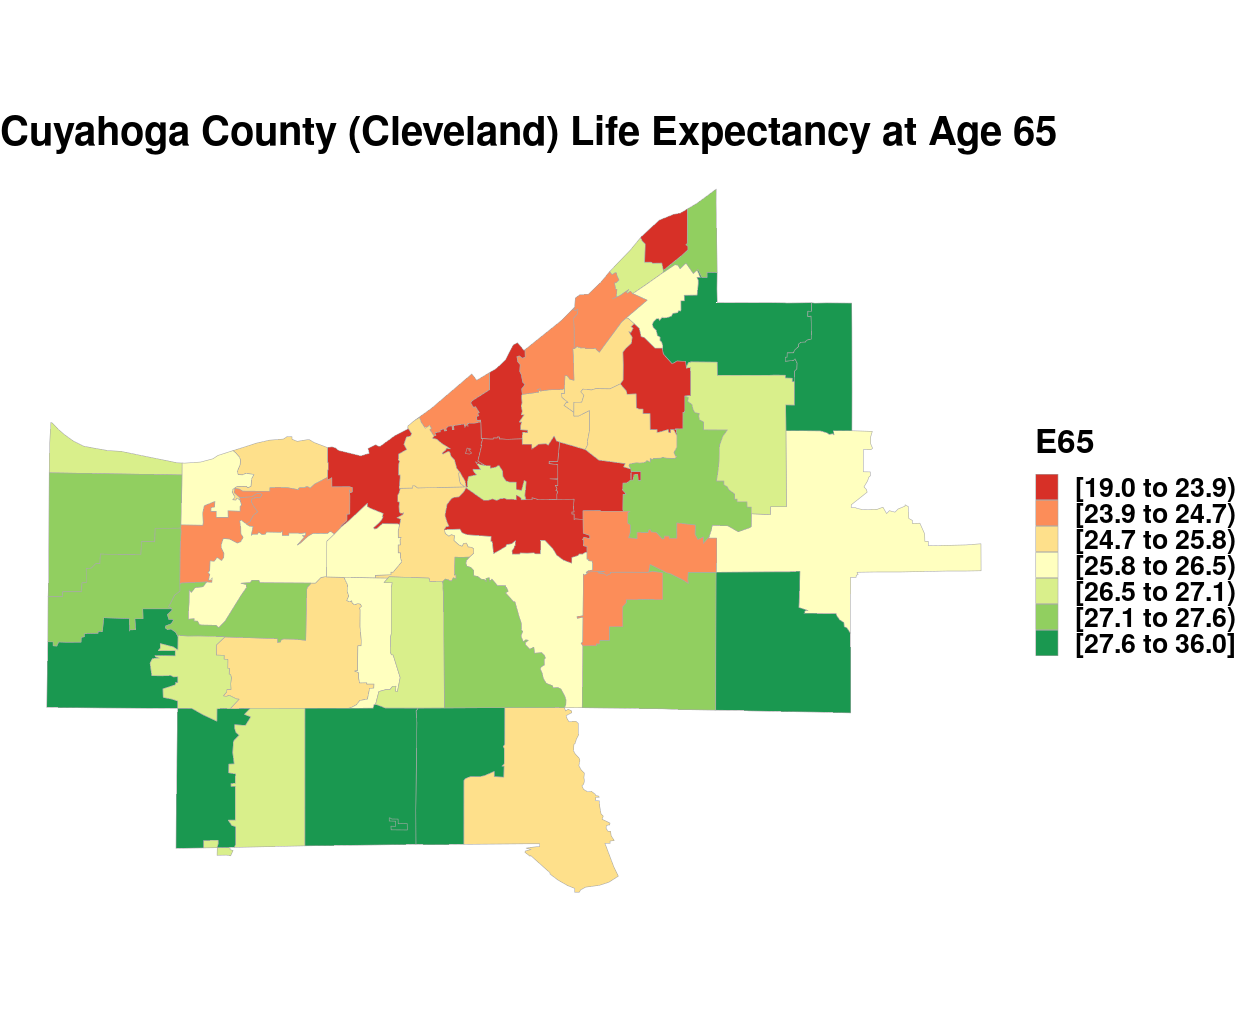
\includegraphics[width=7in]{../illustrations/micro_geography_cleveland.png}
  \caption{Difference in $e65$ in Cuyahoga County for the birth cohorts of 1910-1919}
  \label{fig:cleveland_life_expectancy}
\end{figure}

\hypertarget{gompertz-maximum-likelihood-estimation-race-differentials}{%
\subsubsection{4.5 Gompertz Maximum Likelihood Estimation: Race
Differentials}\label{gompertz-maximum-likelihood-estimation-race-differentials}}

Gompertz maximum likelihood estimation (MLE) can also be used to look at
race differentials in mortality by state in the BUNMD. This method
combines the observed distribution of deaths over a certain window of
deaths with external knowledge of human mortality age-patterns, allowing
us to estimate mortality rates, given a truncated window of deaths
(Alexander 2018). We are assuming that the Gompertz model is appropriate
and that the deaths we observe reflect the true population cohort
distribution. Undercoverage will not bias estimates as long as the
undercoverage is happening at random.

In Figure \ref{fig:gompertz}, we compare estimates of \(e65\) for Whites
and Blacks over time for the cohorts of 1900 to 1920 in the state of
Alabama using a Gompertz model. The size of the BUNMD allows researchers
to identify heterogeneity and identify patterns of mortality obscured by
composite population patterns (Vaupel and Yashin 1985).

\begin{figure}[H]
  \centering
  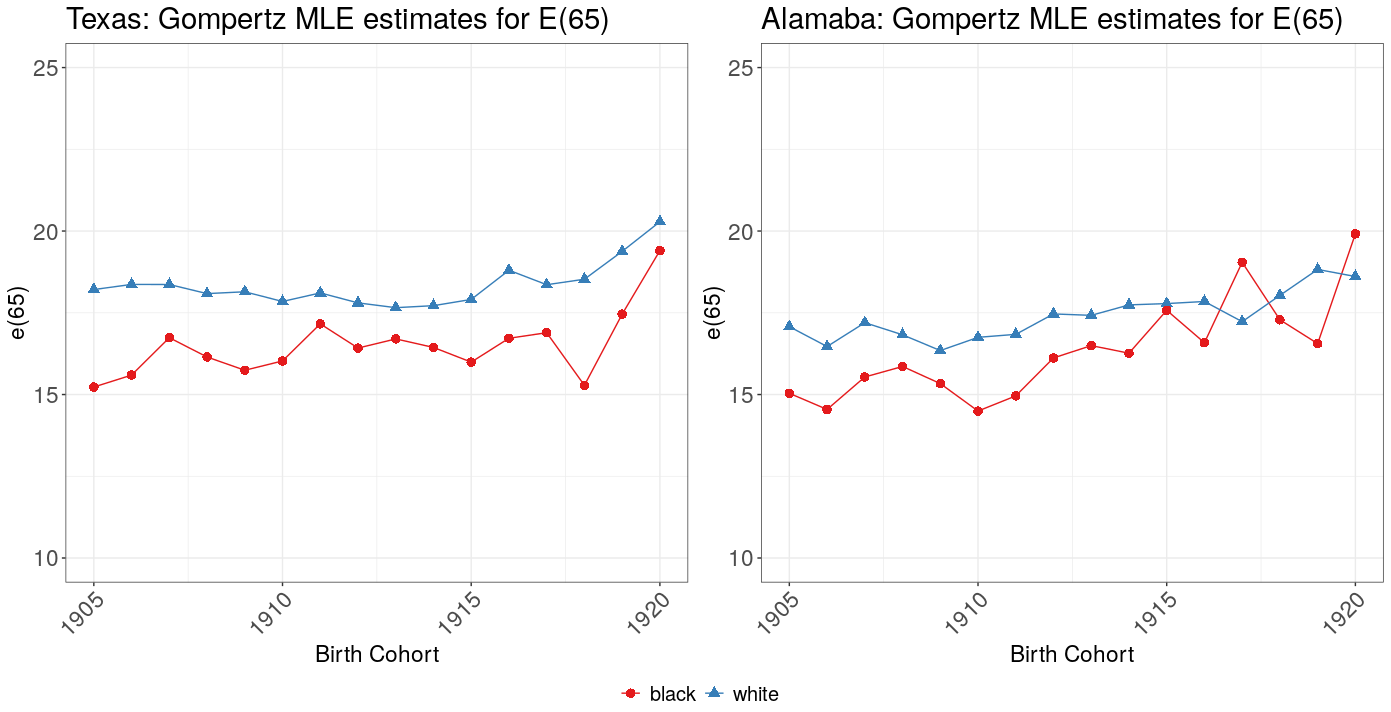
\includegraphics[width=7in]{../illustrations/gompertz_plot.png}
  \caption{Gompertz $e65$ estimates for Alabama for Whites and Blacks.}
  \label{fig:gompertz}
\end{figure}

We chose Alabama and Texas as they had large enough subpopulations,
after disaggregation by birth cohort, for the Gompertz MLE approach to
produce reasonable estimates. Developing diagnostics to assess the fit
of the Gompertz MLE approach and estimate uncertainty is an area for
future research.

\hypertarget{flu-seasons}{%
\subsubsection{4.7 Flu Seasons}\label{flu-seasons}}

The BUNMD's individual death counts by day allows researchers to study
who was hit hardest by the flu, by ZIP Code, race, exact date of birth,
and more. Figure \ref{fig:flu} shows the four US big flu seasons at the
end of the 1990s.

\begin{figure}[H]
  \centering
  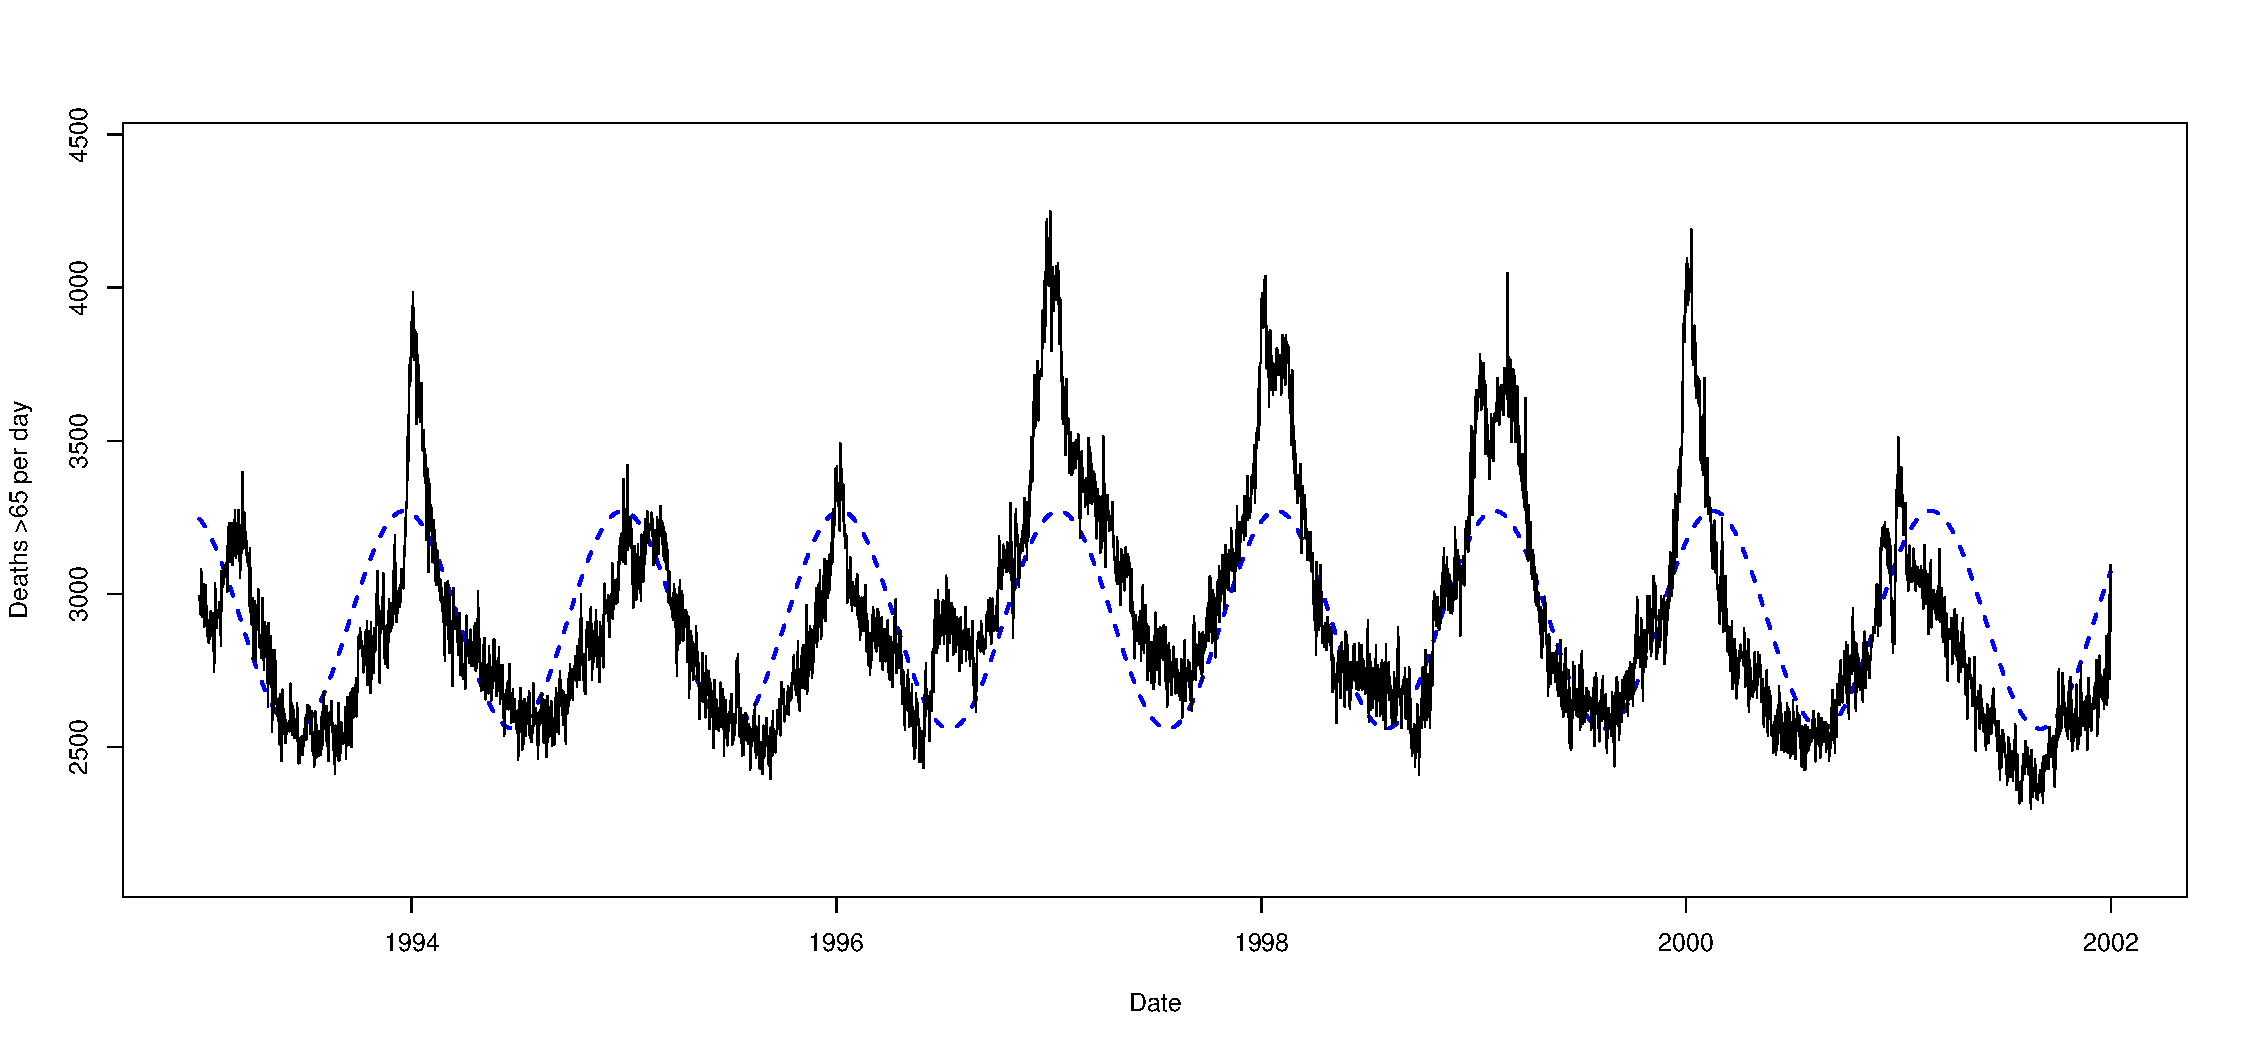
\includegraphics[width=7in]{../illustrations/death_seasonality.pdf}
  \caption{Death counts per day, 1993-2002.}
  \label{fig:flu}
\end{figure}

\hypertarget{conclusion}{%
\subsection{5. Conclusion}\label{conclusion}}

The National Archives release of Numident records has created a new
administrative data resource for researchers studying mortality. We have
created a single-file, cleaned and harmonized version of this data, the
BUNMD, covering more than 49 million deaths. In this paper we have
described the original data and the steps we took to create BUNMD. We
have also provided an overview of statistical methods for estimating
mortality using this deaths-only data set and provided a series of
examples showing how to use the BUNMD. Our hope is that these public
administrative records, with their extraordinary spatial resolution and
size, will open up new avenues for high-resolution mortality research.
Furthermore, we hope that the open-access nature of the data will help
foster research that is reproducible and extendable.

\newpage

\hypertarget{references}{%
\subsubsection*{References}\label{references}}
\addcontentsline{toc}{subsubsection}{References}

\hypertarget{refs}{}
\begin{CSLReferences}{1}{0}
\leavevmode\vadjust pre{\hypertarget{ref-alexander_deaths_2018}{}}%
Alexander, Monica. 2018. {``Deaths Without Denominators: Using a Matched
Dataset to Study Mortality Patterns in the {United} {States}.''}
Preprint. SocArXiv. \url{https://doi.org/10.31235/osf.io/q79ye}.

\leavevmode\vadjust pre{\hypertarget{ref-black_methuselah_2001}{}}%
Black, Dan, (first), Hsu Yu-Chieh, and Lynne Steuerle Schofield. 2001.
{``The {Methuselah} {Effect}: {The} {Pernicious} {Impact} of
{Unreported} {Deaths} on {Old} {Age} {Mortality} {Estimates},''} 45.

\leavevmode\vadjust pre{\hypertarget{ref-chetty_association_2016}{}}%
Chetty, Raj, Michael Stepner, Sarah Abraham, Shelby Lin, Benjamin
Scuderi, Nicholas Turner, Augustin Bergeron, and David Cutler. 2016.
{``The {Association} {Between} {Income} and {Life} {Expectancy} in the
{United} {States}, 2001-2014.''} \emph{JAMA} 315 (16): 1750.
\url{https://doi.org/10.1001/jama.2016.4226}.

\leavevmode\vadjust pre{\hypertarget{ref-gavrilov_mortality_2012}{}}%
Gavrilov, Leonid A, and Natalia S Gavrilova. 2012. {``Mortality
{Measurement} at {Advanced} {Ages}: {A} {Study} of the {Social}
{Security} {Administration} {Death} {Master} {File},''} 26.

\leavevmode\vadjust pre{\hypertarget{ref-goldstein_censoc_2019}{}}%
Goldstein, Joshua .R, Monica Alexander, Casey Breen, Andrea Miranda
González, and Felipe Menares. 2019. {``{CenSoc} {Mortality} {File}:
{Version} 2.0.''} Berkeley: University of California.

\leavevmode\vadjust pre{\hypertarget{ref-goldstein_patrick_2016}{}}%
Goldstein, Joshua R., and Guy Stecklov. 2016. {``From {Patrick} to
{John} {F}.: {Ethnic} {Names} and {Occupational} {Success} in the {Last}
{Era} of {Mass} {Migration}.''} \emph{American Sociological Review} 81
(1): 85--106. \url{https://doi.org/10.1177/0003122415621910}.

\leavevmode\vadjust pre{\hypertarget{ref-greene_censored_2005}{}}%
Greene, William H. 2005. {``Censored {Data} and {Truncated}
{Distributions}.''} \emph{SSRN Electronic Journal}.
\url{https://doi.org/10.2139/ssrn.825845}.

\leavevmode\vadjust pre{\hypertarget{ref-grubesic_use_2006}{}}%
Grubesic, Tony H, and Timothy C Matisziw. 2006. {``On the Use of {ZIP}
Codes and {ZIP} Code Tabulation Areas ({ZCTAs}) for the Spatial Analysis
of Epidemiological Data.''} \emph{International Journal of Health
Geographics} 5 (December): 58.
\url{https://doi.org/10.1186/1476-072X-5-58}.

\leavevmode\vadjust pre{\hypertarget{ref-harper_trends_2014}{}}%
Harper, Sam, Richard F. MacLehose, and Jay S. Kaufman. 2014. {``Trends
{In} {The} {Black}-{White} {Life} {Expectancy} {Gap} {Among} {US}
{States}, 1990--2009.''} \emph{Health Affairs} 33 (8): 1375--82.
\url{https://doi.org/10.1377/hlthaff.2013.1273}.

\leavevmode\vadjust pre{\hypertarget{ref-hill_social_2001}{}}%
Hill, Mark E, and Ira Rosenwaike. 2001. {``The {Social} {Security}
{Administration}'s {Death} {Master} {File}: {The} {Completeness} of
{Death} {Reporting} at {Older} {Ages}.''} \emph{Social Security
Bulletin} 64 (1): 7.

\leavevmode\vadjust pre{\hypertarget{ref-mehta_life_2016}{}}%
Mehta, Neil K., Irma T. Elo, Michal Engelman, Diane S. Lauderdale, and
Bert M. Kestenbaum. 2016. {``Life {Expectancy} {Among} {U}.{S}.-Born and
{Foreign}-Born {Older} {Adults} in the {United} {States}: {Estimates}
{From} {Linked} {Social} {Security} and {Medicare} {Data}.''}
\emph{Demography} 53 (4): 1109--34.
\url{https://doi.org/10.1007/s13524-016-0488-4}.

\leavevmode\vadjust pre{\hypertarget{ref-newby_black_2007}{}}%
Newby, C. Alison, and Julie A. Dowling. 2007. {``Black and {Hispanic}:
{The} {Racial} {Identification} of {Afro}-{Cuban} {Immigrants} in the
{Southwest}.''} \emph{Sociological Perspectives} 50 (3): 343--66.
\url{https://doi.org/10.1525/sop.2007.50.3.343}.

\leavevmode\vadjust pre{\hypertarget{ref-puckett_story_2009}{}}%
Puckett, Carolyn. 2009. {``The {Story} of the {Social} {Security}
{Number}.''} \emph{Social Security Bulletin} 69 (2): 21.

\leavevmode\vadjust pre{\hypertarget{ref-record_group_47_national_archives_numerical_2019}{}}%
Record Group 47, National Archives. 2019. {``Numerical {Identification}
({NUMIDENT}) {Files} {Frequently} {Asked} {Questions}.''} National
Archives; Records Administration.

\leavevmode\vadjust pre{\hypertarget{ref-ruggles_big_2014}{}}%
Ruggles, Steven. 2014. {``Big {Microdata} for {Population}
{Research}.''} \emph{Demography} 51 (1): 287--97.
\url{https://doi.org/10.1007/s13524-013-0240-2}.

\leavevmode\vadjust pre{\hypertarget{ref-scholey_visualizing_2017}{}}%
Schöley, Jonas, and Frans Willekens. 2017. {``Visualizing Compositional
Data on the {Lexis} Surface.''} \emph{Demographic Research} 36
(February): 627--58. \url{https://doi.org/10.4054/DemRes.2017.36.21}.

\leavevmode\vadjust pre{\hypertarget{ref-scott_identifying_1999}{}}%
Scott, Charles G. 1999. {``Identifying the {Race} or {Ethnicity} of
{SSI} {Recipients},''} 12.

\leavevmode\vadjust pre{\hypertarget{ref-vaupel_heterogeneitys_1985}{}}%
Vaupel, James W, and Anatoli I Yashin. 1985. {``Heterogeneity's {Ruses}:
{Some} {Surprising} {Effects} of {Selection} on {Population}
{Dynamics}.''} \emph{The American Statisticiam} 39: 11.

\leavevmode\vadjust pre{\hypertarget{ref-wachter_essential_2014}{}}%
Wachter, Kenneth. 2014. \emph{Essential {Demographic} {Methods}}.
Harvard University Press.

\leavevmode\vadjust pre{\hypertarget{ref-waldron_trends_2007}{}}%
Waldron, Hilary. 2007. {``Trends in {Mortality} {Differentials} and
{Life} {Expectancy} for {Male} {Social} {Security}-{Covered} {Workers},
by {Socioeconomic} {Status}.''} \emph{Social Security Bulletin} 67 (3):
28.

\end{CSLReferences}

\newpage

\hypertarget{technical-appendix}{%
\section{Technical Appendix}\label{technical-appendix}}

This supplementary appendix presents the procedure for constructing the
Berkeley Unified Numident Mortality Database (BUNMD) from the original
NARA Numident records. Please see the BUNMD Codebook for variable
descriptions, value labels, and tabulations.

\hypertarget{nara-numident-records}{%
\subsection{1.1 NARA Numident Records}\label{nara-numident-records}}

In 2013, the Social Security Administration transferred a set of
Numident records to the National Archives (NARA). In 2019, we obtained
the NARA Numident records and their accompanying documentation. The NARA
Numident records are a subset of the records in the complete Numident.
The NARA Numident records contain three types of entries: application,
claim, and death. NARA delivered each set of entries separately as a set
20 fixed-width .txt files (3 x 20 = 60 files in total).

\hypertarget{nara-numident-metadata}{%
\subsection{1.2 NARA Numident Metadata}\label{nara-numident-metadata}}

We obtained three documents from the National Archives Technical
Documentation series:

(\url{https://aad.archives.gov/aad/popup-tech-info.jsp?s=5057}; accessed
11/28/2019):

\begin{itemize}
\tightlist
\item
  Application (SS-5) Records Layout
\item
  Death Records Layout
\item
  Claim Records Layout
\end{itemize}

The record layout documents contain variable descriptions, value labels,
technical notes, and the start and end position for each variable in the
60 fixed-width .txt files.

\hypertarget{code}{%
\subsection{1.3 Code}\label{code}}

All data processing was was done in the \texttt{R} Statistical
Programming Language. The code to construct the BUNMD from the NARA
Numident records is available at ``Github.com/caseybreen/wcensoc/.''

\hypertarget{data-preprocessing}{%
\subsection{1.4 Data Preprocessing}\label{data-preprocessing}}

For each of the three entry types, we read in the 20 fixed-width .txt
files using the column position specified in the record layout
documents. We then appended the 20 files into a single file, creating a
single file for each of the three entry types.

We took the following steps to clean each file:

\begin{enumerate}
\def\labelenumi{\arabic{enumi}.}
\item
  We changed the variable names to be more concise and informative. For
  example, we renamed the ``NUMI\_SEX'' variable to ``sex.''
\item
  We harmonized the different codes to represent a missing value
  (``Unknown,'' ``Unk,'' ``Un,'' and ``0'') to ``NA.''
\end{enumerate}

\hypertarget{combining-nara-numident-records-into-the-bunmd}{%
\subsection{1.5 Combining NARA Numident Records into the
BUNMD}\label{combining-nara-numident-records-into-the-bunmd}}

The goal in constructing the BUNMD was to combine the NARA Numident
records into a single, harmonized file with one record per person. The
original records contain over 100+ variables. Some are not of general
interest to the research community, while others contain 99\%+ missing
values (as shown in Figures 2-4). We selected a set of general-interest
variables with high completeness.

While a person can only have one death entry, they might have several
application or claim entries; information may be reported several times.
For example, sex is reported in the application, claim, and death
entries. Occasionally, a person reports different values of sex, race,
place of birth, etc. across entries. To handle this response
inconsistency, we developed a set of decision rules to select a single
value across entries (see Table 2). In order to study name changes, race
changes, and other features, the original NARA Numident records are
useful and are available upon request.

\hypertarget{geography-1}{%
\subsection{1.6 Geography}\label{geography-1}}

\textbf{Place of Birth:} There are several geographic variables in the
NARA Numident records. The application entries have information on
birthplace. For persons born in the United States, the geographic
resolution is state-level. For persons born outside the United States,
the geographic resolution is country-level. The NARA Numident uses two
variables to convey birthplace. The first variable denotes whether a
person was foreign born, and the second variable contains a two-letter
state or country abbreviation. We harmonize these two variables into one
variable with a numeric coding schema. This coding schema matches the
IPUMS-USA BPLD (Birthplace, detailed) schema.

\textbf{Place of Death:} The Numident death entry contains the 9-digit
ZIP Code of the residence at the time of death. Sometimes, the full
9-digit ZIP Code is not available, and an ``x'' is used to represent a
missing digit. This is the original convention used by the Social
Security Administration.

\textbf{Social Security State:} The first three digits of a Social
Security number correspond to the state in which a Social Security
number was issued (prior to 1973) or to the ZIP Code of the mailing
address listed in the Social Security application (after 1973). We
constructed a variable ``socstate'' that reports the the state
corresponding to the first three digits of the Social Security number.
The Social Security Administration changed the assignment process in
2011 --- after the last Social Security number for a person in the BUNMD
was issued --- and the first three digits no longer correspond to a
state.

(\url{https://www.ssa.gov/employer/stateweb.htm}; accessed 11/28/2019)

\begin{figure}
  \centering
  \subfloat[\label{fig:tp01}]{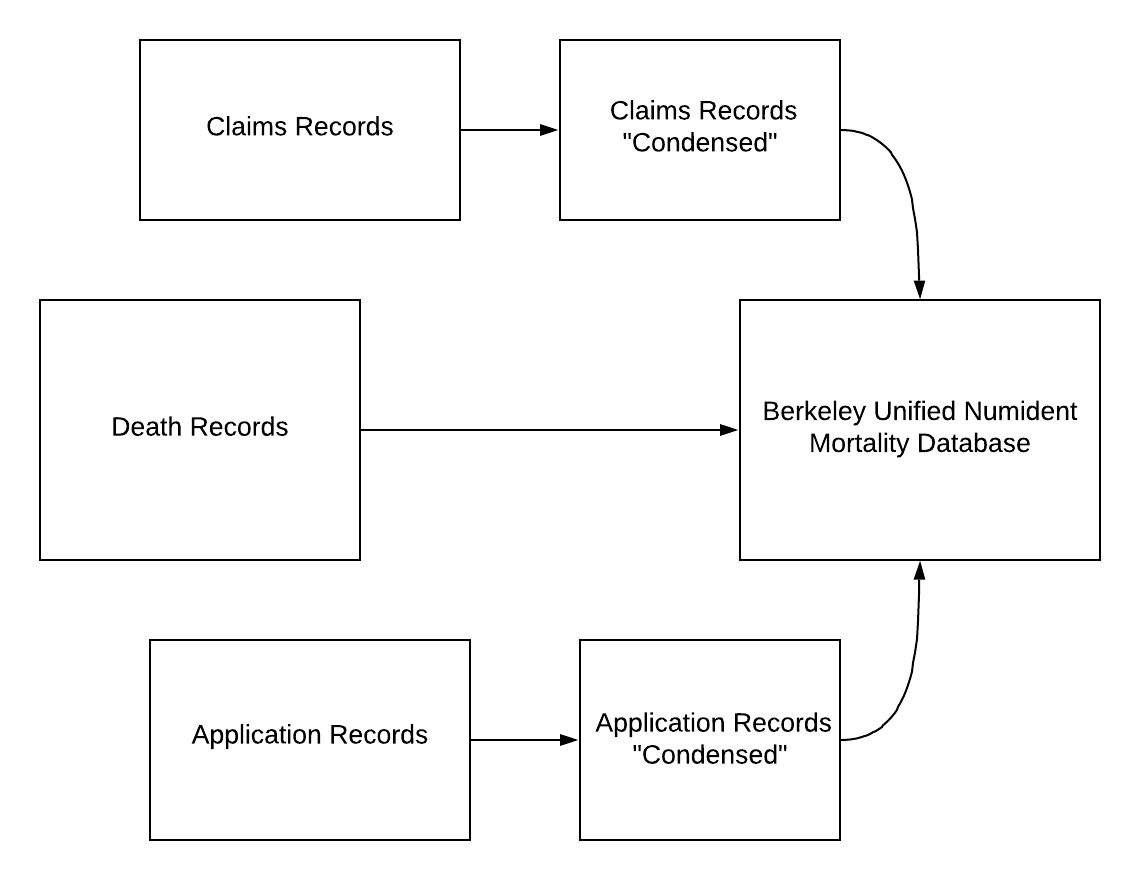
\includegraphics[width=5.5in]{../illustrations/numident_flowchart.png}}
  \caption{BUNMD Construction Flow Chart}
  \label{fig:tp}
\end{figure}

\newpage

\hypertarget{bunmd-samples-and-weights}{%
\subsection{1.7 BUNMD Samples and
Weights}\label{bunmd-samples-and-weights}}

We created two BUNMD samples with high death coverage. Sample 1 includes
deaths to persons with high coverage (age 65+), occurring between 1988
to 2005, from the birth cohorts of 1900 to 1940. Sample 2 is the subset
of Sample 1 records with complete information on sex, birthplace, and
race. For each sample, we constructed inverse probability weights to the
Human Mortality Database (HMD) on age at death, year of birth, year of
death, and sex. We broke the sample into cells cross-classified by year
of birth, year of death, age at death, and sex. We weighted each cell to
the HMD ``Deaths by Lexis triangles'' totals. This allows aggregation to
HMD totals by period or cohort.

\begin{equation}
  W_j = \frac{\text{HMD deaths in cell j}}{\text{Numident Sample 1 deaths in cell j}} 
\end{equation}

\newpage

\textbf{\large Decision Rules used for BUNMD}

\begin{longtable}[]{@{}lll@{}}
\toprule
Variable & Numident Source & Selection Rule \\
\midrule
\endhead
ssn & Death Entry & - \\
fname & Death Entry & - \\
mname & Death Entry & - \\
lname & Death Entry & - \\
byear & Death Entry & - \\
bmonth & Death Entry & - \\
bday & Death Entry & - \\
dyear & Death Entry & - \\
dmonth & Death Entry & - \\
dday & Death Entry & - \\
zip\_residence & Death Entry & - \\
sex & Death, Application, or Claim Entry & Last Recorded Sex \\
race\_first & Application Entry & First Recorded Race \\
race\_last & Application Entry & Last Recorded Race \\
bpl & Application or Claim Entry & Last Recorded BPL \\
father\_fname & Application or Claim Entry & Maximum Characters \\
father\_mname & Application or Claim Entry & Maximum Characters \\
father\_lname & Application or Claim Entry & Maximum Characters \\
mother\_fname & Application or Claim Entry & Maximum Characters \\
mother\_mname & Application or Claim Entry & Maximum Characters \\
mother\_lname & Application or Claim Entry & Maximum Characters \\
race\_change & Constructed & - \\
death\_age & Constructed & - \\
socstate & Constructed & - \\
age\_first\_app & Constructed & - \\
number\_apps & Constructed & - \\
number\_claims & Constructed & - \\
weight & Constructed & - \\
ccweight & Constructed & - \\
\bottomrule
\end{longtable}

Table 1: The selection rules used to construct the BUNMD. For a given
variable, we selected values from the death record, if available. If a
value wasn't available in the death record, we chose a value from the
application record using selection rules. If it was not available in
either the death or application entry, we selected it from the claim
record.

\newpage

\begin{figure}
  \centering
  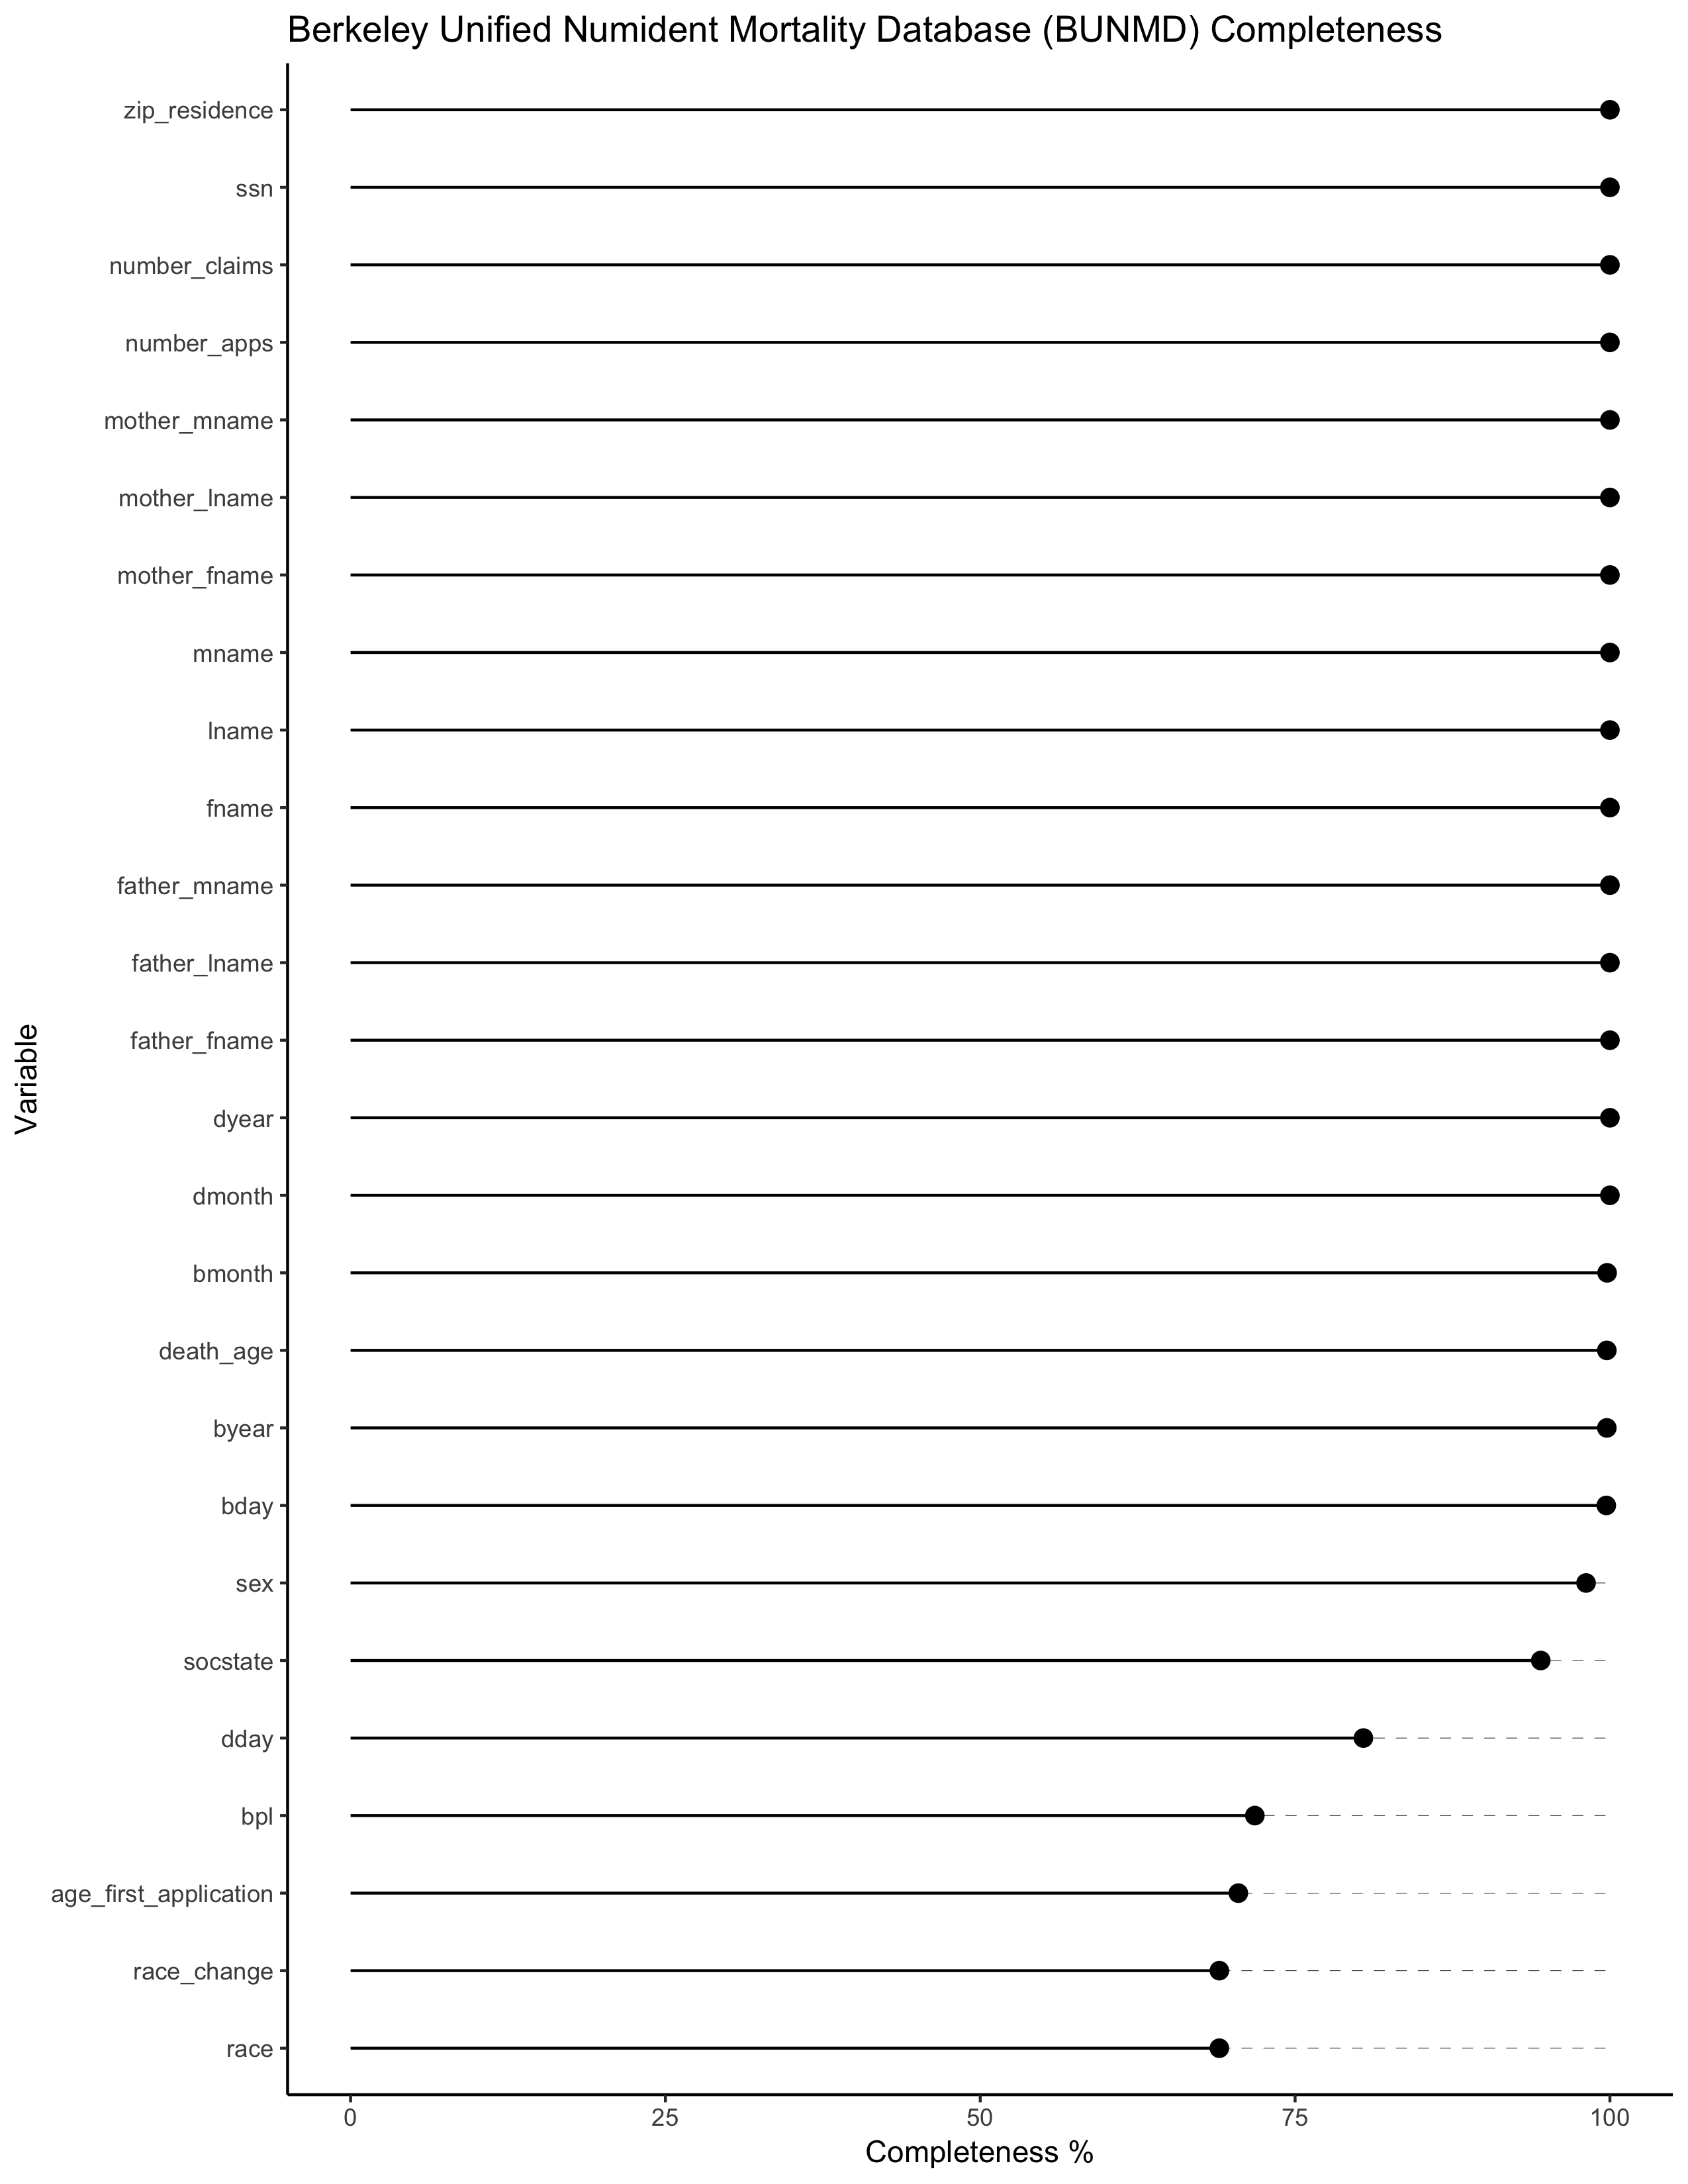
\includegraphics[width = 6.9in]{../illustrations/bunmd_coverage_completeness.png}
  \caption{}
\end{figure}

\begin{figure}
  \centering
  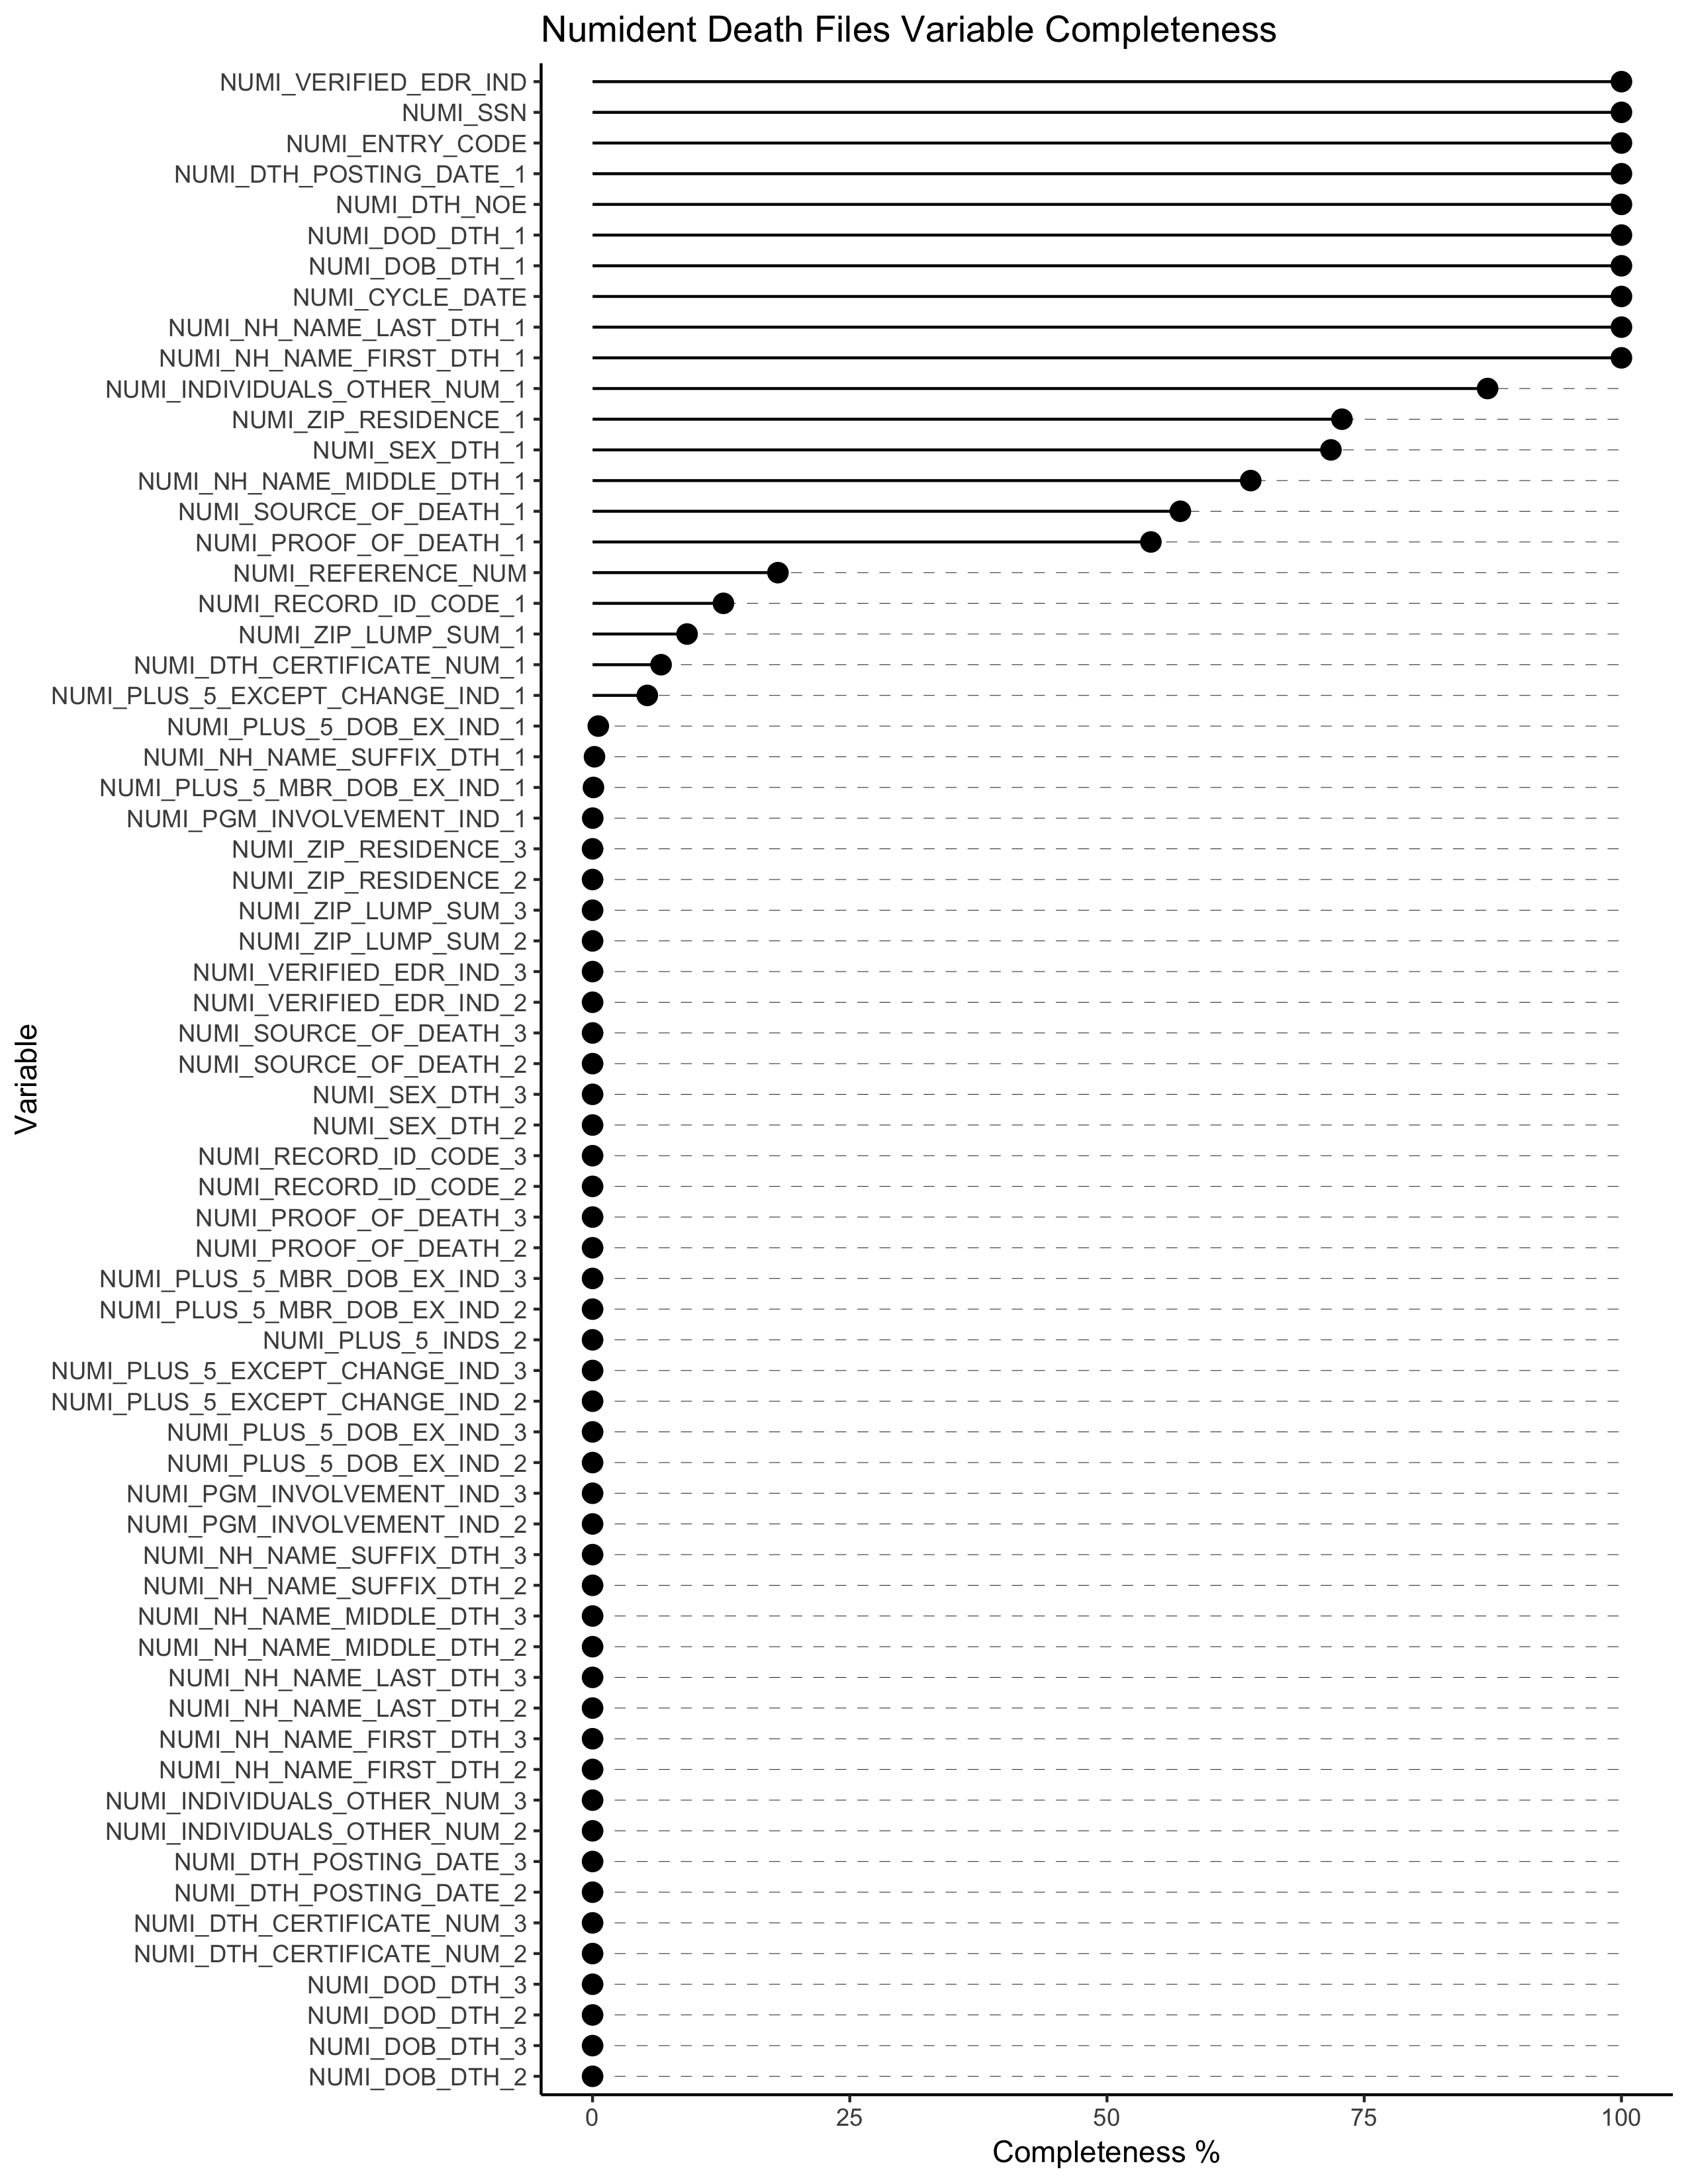
\includegraphics[width = 6.9in]{../illustrations/death_coverage.png}
  \caption{}
\end{figure}

\begin{figure}
  \centering
  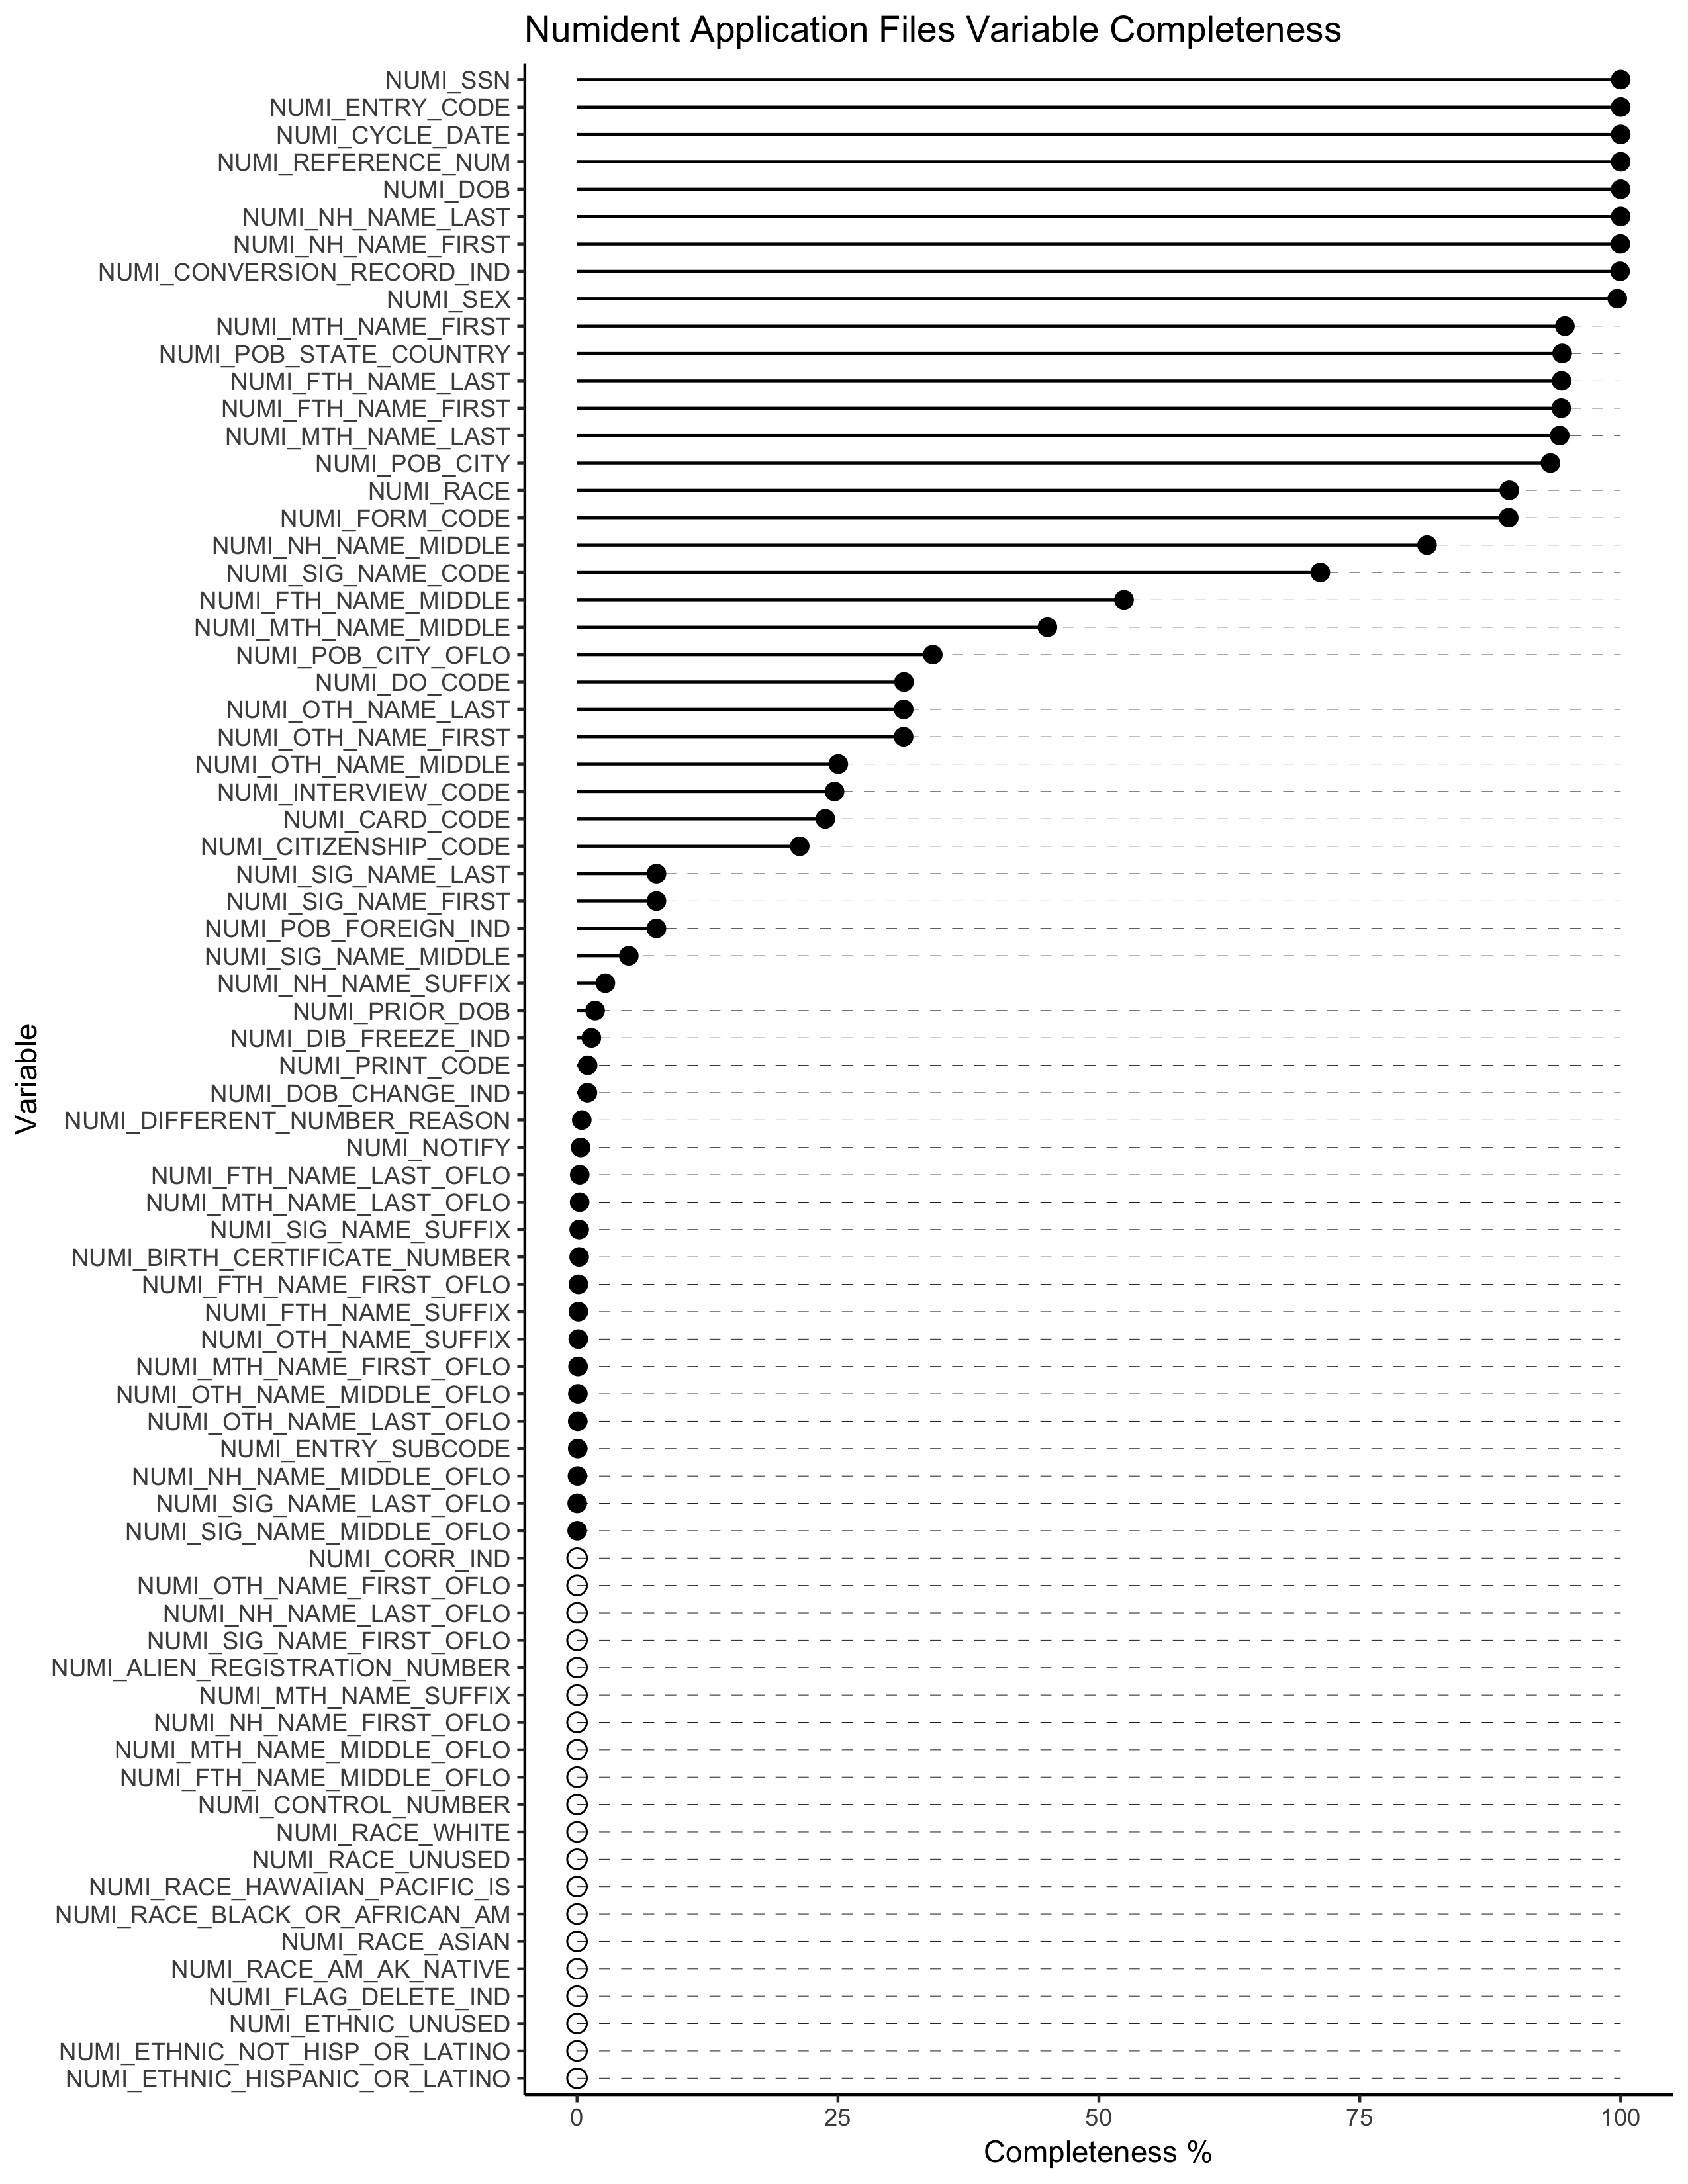
\includegraphics[width = 6.9in]{../illustrations/application_coverage.png}
  \caption{}
\end{figure}

\begin{figure}
  \centering
  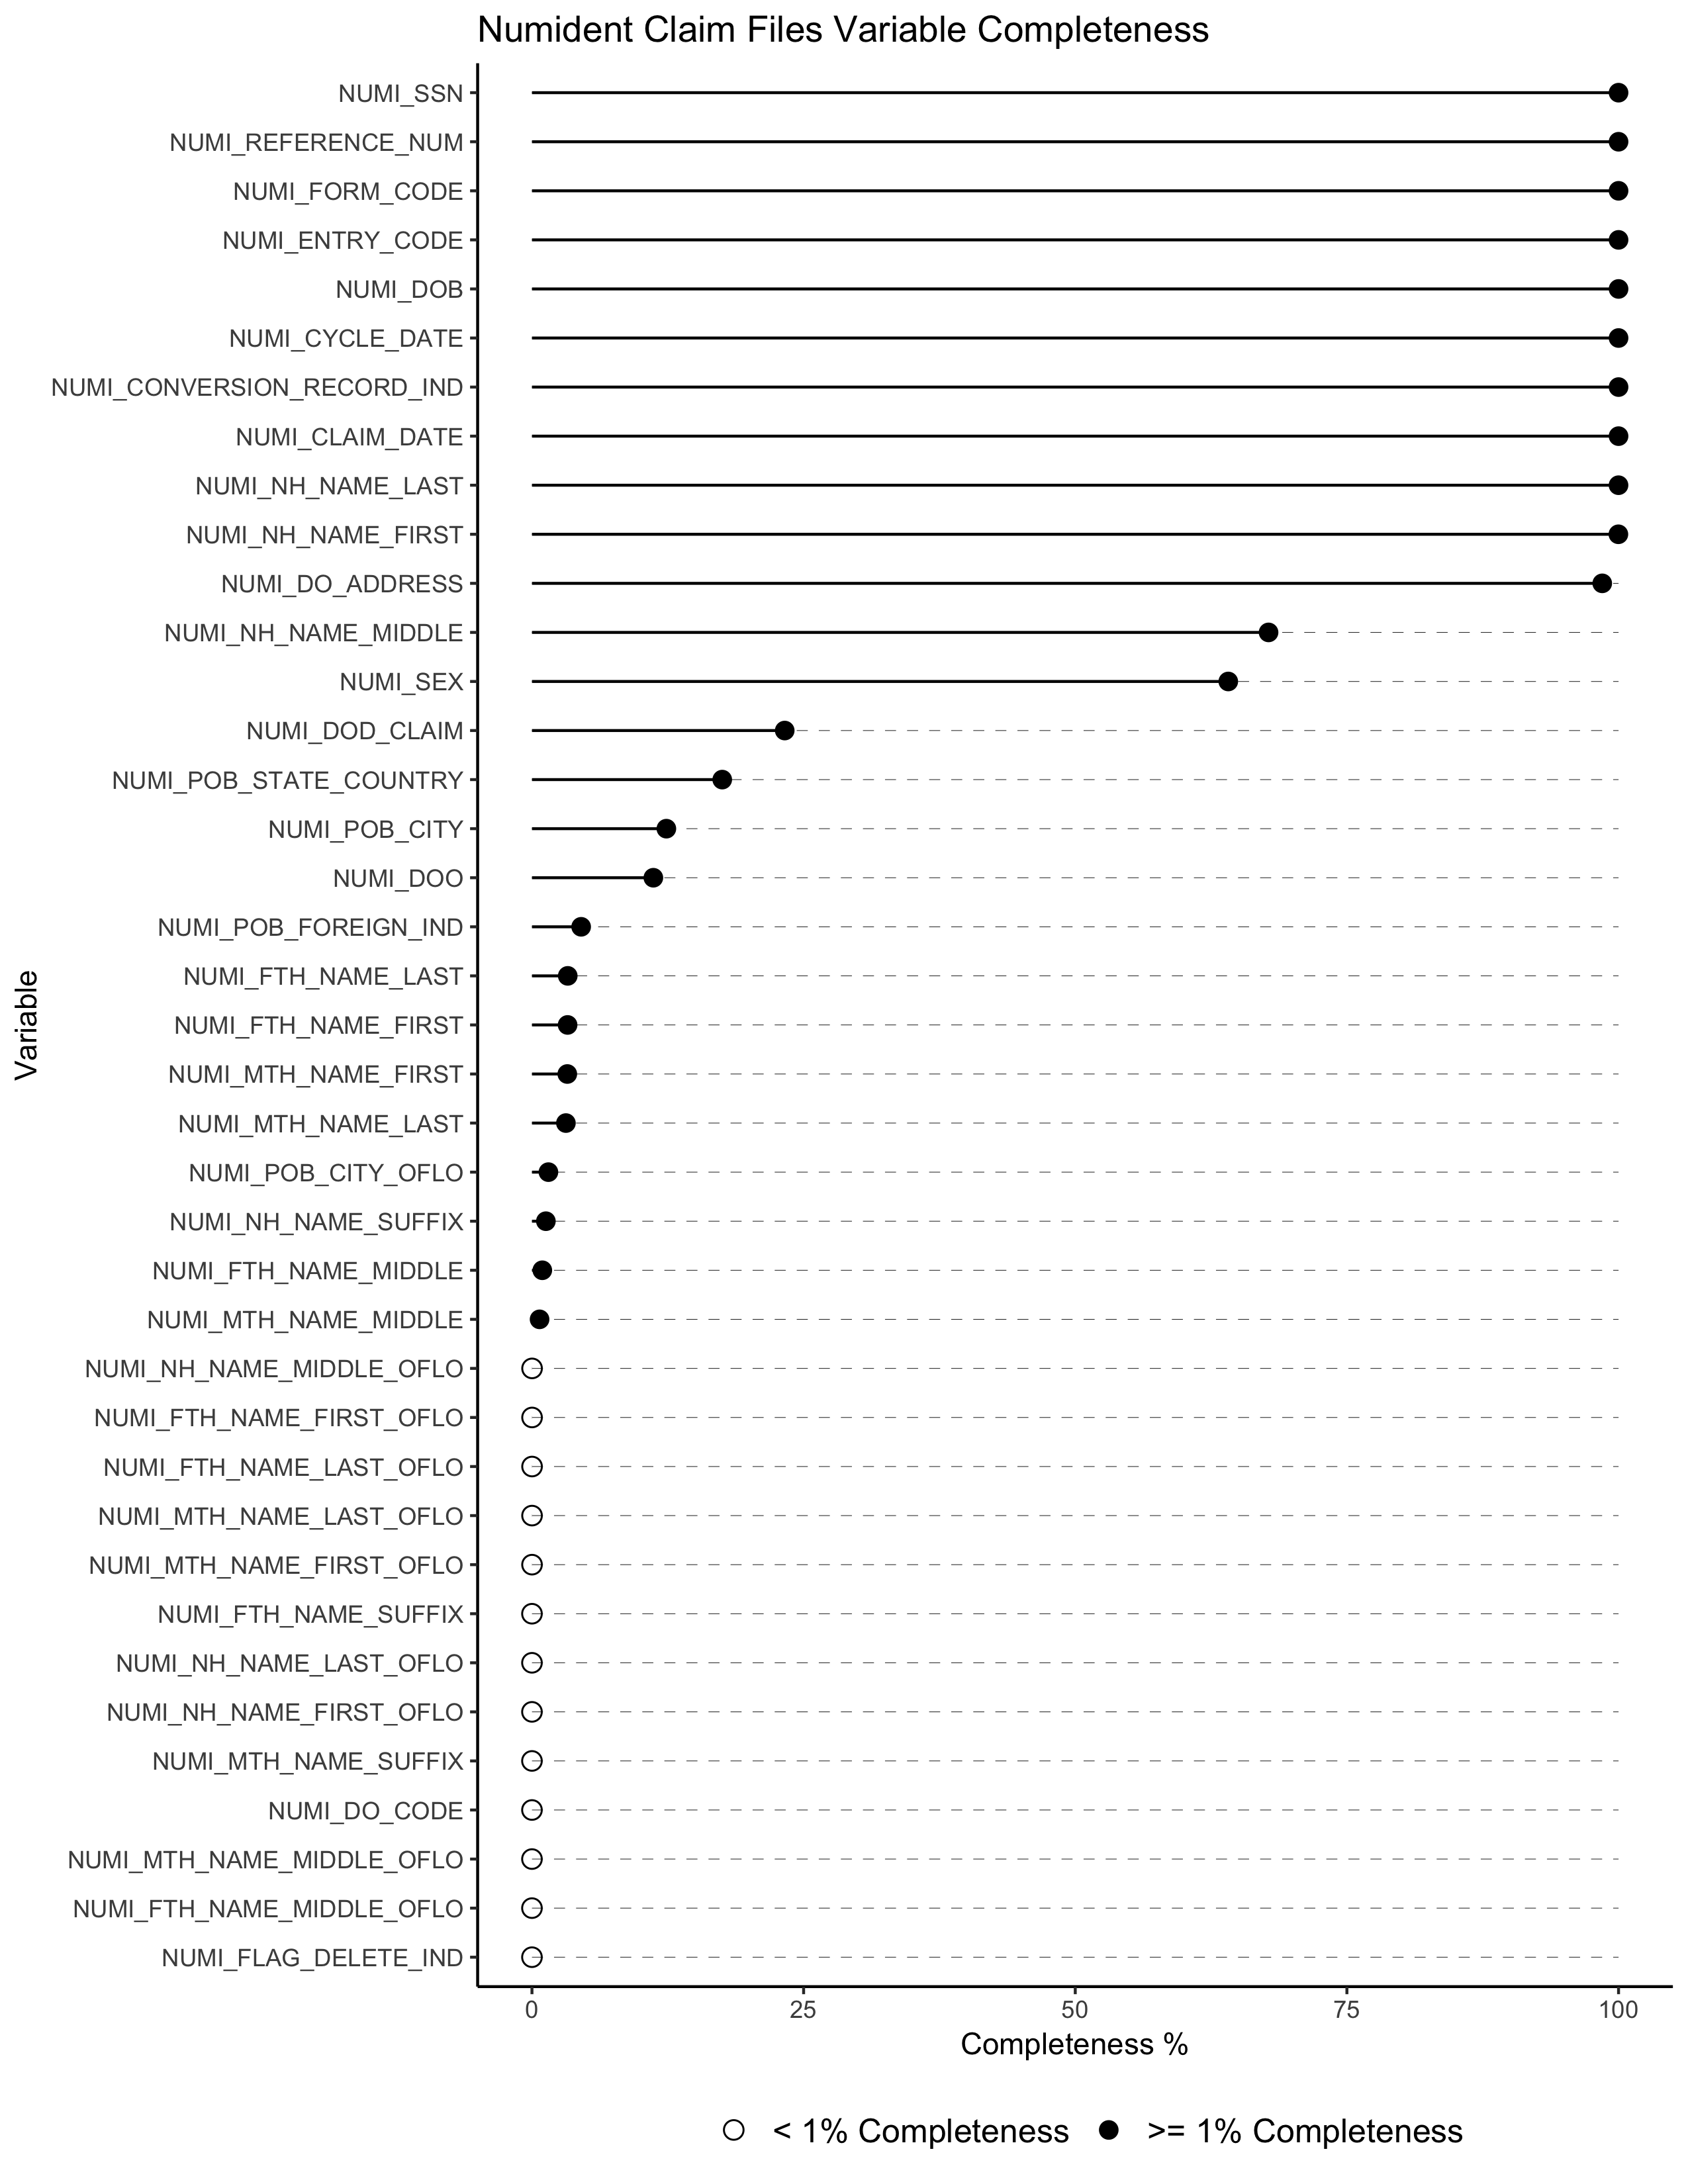
\includegraphics[width=6.9in]{../illustrations/claim_coverage.png}
  \caption{}
\end{figure}

\newpage

\end{document}
